\documentclass[mat1]{fmfdelo}
% \documentclass[fin1]{fmfdelo}
% \documentclass[isrm1]{fmfdelo}
% \documentclass[mat2]{fmfdelo}
% \documentclass[fin2]{fmfdelo}
% \documentclass[isrm2]{fmfdelo}

% naslednje ukaze ustrezno napolnite
\avtor{Lenart Treven}

\naslov{Metode podpornih vektorjev}
\title{Support vector machines}

% navedite ime mentorja s polnim nazivom: doc.~dr.~Ime Priimek,
% izr.~prof.~dr.~Ime Priimek, prof.~dr.~Ime Priimek
% uporabite le tisti ukaz/ukaze, ki je/so za vas ustrezni
\mentor{doc.~dr.~Matija Pretnar}
% \mentorica{}
 \somentor{dr.~Jan Kralj}
% \somentorica{}
% \mentorja{}{}
% \mentorici{}{}

\letnica{2018} % leto diplome

%  V povzetku na kratko opišite vsebinske rezultate dela. Sem ne sodi razlaga organizacije dela --
%  v katerem poglavju/razdelku je kaj, pač pa le opis vsebine.
\povzetek{V delu predstavimo metode podpornih vektorjev, njihovo matematično izpeljavo in pra\-kti\-čno uporabo. Izpeljemo primarni problem, ki ga dobimo, ko želimo linearno ločljive dvorazredne podatke ločiti s hiperravnino. Dani problem posplošimo na dvorazredne podatke, ki niso linearno ločljivi. Predstavimo teorijo dualnosti konveksnih optimizacijskih problemov, s pomočjo katere dokažemo krepki izrek o dualnosti za konveksne probleme. Primarni problem prevedemo na njegov dual. V dualni problem uvedemo jedrne funkcije. Dokažemo, da sta polinomsko in radialno jedro skalarna produkta. Pokažemo, kako ravnamo v primeru, ko imamo večrazredne podatke. Pokažemo način, kako ocenimo natančnost klasifikatorja s prečnim preverjanjem. Pokažemo delovanje različnih jeder na preprostih dvorazsežnih podatkih, ki jih vzamemo iz podatkovne množice IRIS. Metode podpornih vektorjev naučimo na večji podatkovni množici ter pokažemo, na kakšen način izberemo končni napovedni model. }

%  Prevod slovenskega povzetka v angleščino.
\abstract{In this work we present support vector machines, their mathematical derivation and practical usage. The primal problem, which we encounter while trying to separate two-class data with hyperplane, is described. We generalise given primal problem to nonlinear separable data. The theory of convex optimization is introduced which helps us to prove strong duality in the convex case. We convert the primal problem to its dual. Kernel functions are introduced into the dual problem. We prove that the polynomial and radial kernels are scalar products in some space. The problem of multiclass data is described. Methods such as cross-validation are introduced for error estimation. Different kernels are demonstrated on a simple two dimensional data set, which is a part of the IRIS data set. Support vector machines are trained on a bigger data set and an indication of a possible way of choosing final model is shown.}

% navedite vsaj eno klasifikacijsko oznako --
% dostopne so na www.ams.org/mathscinet/msc/msc2010.html
\klasifikacija{49N15, 	68T01 }
\kljucnebesede{metode podpornih vektorjev, dualni problem, jedra} % navedite nekaj ključnih pojmov, ki nastopajo v delu
\keywords{support vector machines, dual problem, kernel functions} % angleški prevod ključnih besed

\zapisiMetaPodatke  % poskrbi za metapodatke in veljaven PDF/A-1b standard

% aktivirajte pakete, ki jih potrebujete
\usepackage{minted}
\usepackage{enumerate} 
\usepackage{dsfont}
\usepackage{algorithm}
\usepackage{algorithmicx}
\usepackage{algpseudocode}
\usepackage{makecell}
\usepackage{subcaption}
\usepackage{graphicx}
\usepackage{booktabs}
\usepackage{siunitx}




% za številske množice uporabite naslednje simbole
\newcommand{\R}{\mathbb R}
\newcommand{\N}{\mathbb N}
\newcommand{\Z}{\mathbb Z}
\newcommand{\C}{\mathbb C}
\newcommand{\Q}{\mathbb Q}



% matematične operatorje deklarirajte kot take, da jih bo Latex pravilno stavil
% \DeclareMathOperator{\conv}{conv}
\DeclareMathOperator{\sign}{sign}
\DeclareMathOperator{\diag}{diag}
\DeclareMathOperator{\Int}{Int}
\DeclareMathOperator{\Cl}{Cl}
\DeclareMathOperator{\dom}{dom}

% vstavite svoje definicije ...
%  \newcommand{}{}
\newcommand{\pr}{\mathbf 1}
\newcommand{\nr}{\mathbf {-1}}

\begin{document}

\section{Uvod}

Metode podpornih vektorjev sodijo v področje nadzorovanega strojnega učenja. Z njimi si pomagamo, ko želimo s pomočjo že znanih podatkov napovedati razrede novim podatkom.  Kot primer si lahko predstavljamo, da smo opravili meritve listov različnih rož, biolog pa nam je povedal, katerim vrstam te rože pripadajo. S pomočjo metod podpornih vektorjev bi na podlagi že znanih meritev in meritve lista nove rože lahko napovedali, v kateri razred spada posamezna roža, ne da bi pri tem vprašali biologa.

V diplomskem delu problem najprej prevedemo v matematični jezik. V poglavjih \ref{dual}, \ref{updual}, in \ref{PoglavjeMetodeJeder} predstavimo teoretično ozadje problema. V poglavju \ref{poglavjePrimerUporabe} pa si ogledamo primer uporabe metod podpornih vektorjev. Uvodno poglavje \ref{poglavjeOpisProblema} sledi literaturi \cite[str. 337--356]{DM}, \cite[str. 417--426]{ESL} in \cite[str. 214--235]{AITSL}. Pri poglavjih \ref{dual}, \ref{updual} smo sledili \cite{ITNO}. V poglavju \ref{poglavjePrimerUporabe} prikažemo rezultate, ki smo jih dobili z lastno implementacijo. 


\section{Opis problema}
\label{poglavjeOpisProblema}

\subsection{Predstavitev podatkov}
V tem razdelku bomo predstavili, s kakšnimi podatki se ukvarjamo ter kako jih predstavimo. 
Oglejmo si znan primer s področja strojnega učenja. Izvajamo meritve treh različnih vrst rož. Vsaki posamezni roži izmerimo dolžino in širino venčnega in čašnega lista. Biolog nam dodatno pove, katera vrsta rože je merjena rastlina. Skupaj imamo $5$ podatkov o vsaki roži. V tem primeru so podatki elementi prostora $\R^4 \times Y$, kjer so meritve zbrane v $\R^4$, kateri vrsti pripada meritev, pa nam pove podatek iz $Y$. V splošnem podatke predstavimo kot elemente prostora $\R^n \times Y$, kjer je $n$ numeričnih meritev zbranih v vektorju iz $\R^n$, pripadajoči razredi pa so elementi v $Y$. Na začetku se bomo ukvarjali s primerom, ko podatki pripadajo dvema razredoma. Ta dva razreda bomo poimenovali $\nr$ in $\pr$. Kasneje bomo obravnavali tudi primer, ko imamo opravka s podatki, ki pripadajo več razredom. Množico $m$ podatkov predstavimo z \emph{matriko podatkov} $X \in \R^{m \times n}$ s pripadajočim \emph{vektorjem razredov} $y \in \R^m$. Vrstica $i$ predstavlja $i$-to meritev, $i$-ti element vektorja $y$ pa pove, kateremu razredu pripada $i$-ta meritev. 
\begin{primer}
	Recimo, da imamo meritve: $x_1 = (1,6,-2)^T, x_2 = (-2, 7, 2)^T, x_3 = (-1,-2,-3)^T, x_4 = (\frac{4}{3}, 5, 0)^T$, s pripadajočimi razredi $x_1, x_4 \in \pr, x_2, x_3 \in \nr$. Predstavimo jih kot: 
	\begin{align*} X =  
	\begin{bmatrix}
	1 & 6 & -2  \\
	-2 & 7 &  2     \\
	-1 & -2 & -3  \\
	\frac{4}{3}& 5 & 0 
	\end{bmatrix}, y=\begin{bmatrix}
	1   \\
	-1    \\
	-1 \\
	1
	\end{bmatrix}. &\qedhere
	\end{align*}
\end{primer}

\begin{opomba}
	Včasih bomo samim meritvam $X \in \R^{m \times n}$ rekli podatki, $y \in Y^m$ pa bomo rekli pripadajoči vektor razredov. 
\end{opomba}
\subsection{Linearno ločljivi podatki}

Za začetek se omejimo na tako imenovane linearno ločljive podatke, ki pripadajo dvema razredoma. Naš cilj je poiskati čim boljšo mejo med podatki, ki pripadajo različnima razredoma. 

\begin{definicija}
	\emph{Hiperravnina} v $\R^n$ je $n - 1$ razsežen afin podprostor. 
\end{definicija}
Hiperravnino v  $\R^n$ lahko predstavimo kot množico rešitev enačbe $$ w_1x_1 + w_2x_2 + \cdots + w_nx_n + b = 0,$$ kjer so $b$ in $w_i, $ za $ i = 1,\ldots,n $ znani koeficienti, $x_i$ pa spremenljivke. Pri tem mora tudi veljati, da je vsaj en $w_i$ različen od $0$. Kompaktneje to lahko zapišemo kot $w^Tx  + b = 0$. Za vsako točko $a \in \R^n$ velja, da bodisi $w^Ta  + b > 0$ bodisi $w^Ta+ b < 0$ bodisi $w^Ta+ b = 0$. 

\begin{definicija}
	Pravimo, da so podatki $(X, y)$ \emph{linearno ločljivi}, če obstaja hiperravnina, določena z enačbo $w^Tx+ b = 0$, tako da za vsak $i$ velja:
	$y_i = 1 \implies w^Tx_i+ b > 0$,  $y_i = -1 \implies w^Tx_i+ b < 0$, kjer smo z $x_i$ označili $i$-to vrstico matrike podatkov $X$, z $y_i$ pa $i$-to komponento vektorja pripadajočih razredov $y$.
\end{definicija} 

Zgornjo definicijo si lahko predstavljamo tako, da hiperravnina razdeli $\R^n$ na dve polovici. Če podatek pripada razredu $\pr$, potem leži ``nad'' to hiperravnino, če pa pripada razredu $\nr$, potem leži ``pod'' to hiperravnino.  Če že imamo podano hiperravnino, lahko definiramo funkcijo $r(x) = w^Tx+ b$, ki pove, kje se podatek $x$ nahaja v prostoru. Če je vrednost funkcije v točki $x$ negativna, leži pod hiperravnino, če je enaka nič, leži na hiperravnini, če je večja od nič, pa leži nad hiperravnino. Funkcija $|r|$ podaja razdaljo točk do izbrane hiperravnine, pomnoženo še z normo vektorja $w.$ 

\begin{definicija}
	\emph{Klasifikator} $f: \R^n \to Y$ je funkcija, ki dani točki v $\R^n$ priredi neki razred v $Y$.
\end{definicija}

Lotimo se sedaj našega cilja, izdelave klasifikatorja s pomočjo hiperravnine. Recimo, da imamo linearno ločljive podatke, ki jih loči hiperravnina $(w, b)$. Tedaj lahko zapišemo klasifikacijsko funkcijo kot: 
$$ f(x) = \sign{(w^Tx+ b)}.$$
Vsem točkam, ki ležijo na zgornji strani hiperravnine, smo pripisali razred $\pr$, in obratno, točkam na spodnji strani hiperravnine pripišemo razred $\nr$. Tako zelo enostavno klasificiramo nove podatke. 

Takih ločnih ravnin (in posledično klasifikacij) je lahko več. Vprašanje je, katero izmed vseh možnih izbrati. Pri tej odločitvi bo ključnega pomena minimalna evklidska oddaljenost že znanih točk posameznega razreda od hiperravnine. Hiperravnino $\Pi = (w, b)$ bomo izbrali tako, da bodo izpolnjeni naslednji pogoji: 
\begin{enumerate}[(i)]
	\item 
	Za vse točke iz razreda $\pr$, bo veljalo $w^Tx+ b > 0$.
	\item 
	Za vse točke iz razreda $\nr$, bo veljalo $w^Tx+ b < 0$.
	\item 
	Minimalna razdalja točk razreda $\pr$ do hiperravnine $\Pi$ bo enaka minimalni razdalji točk razreda $\nr$ do $\Pi$.
	\item 
	Ta razdalja naj bo maksimalna med vsemi ravninami, ki ločijo podatke.
\end{enumerate}
\begin{figure}[H]
	\centering
	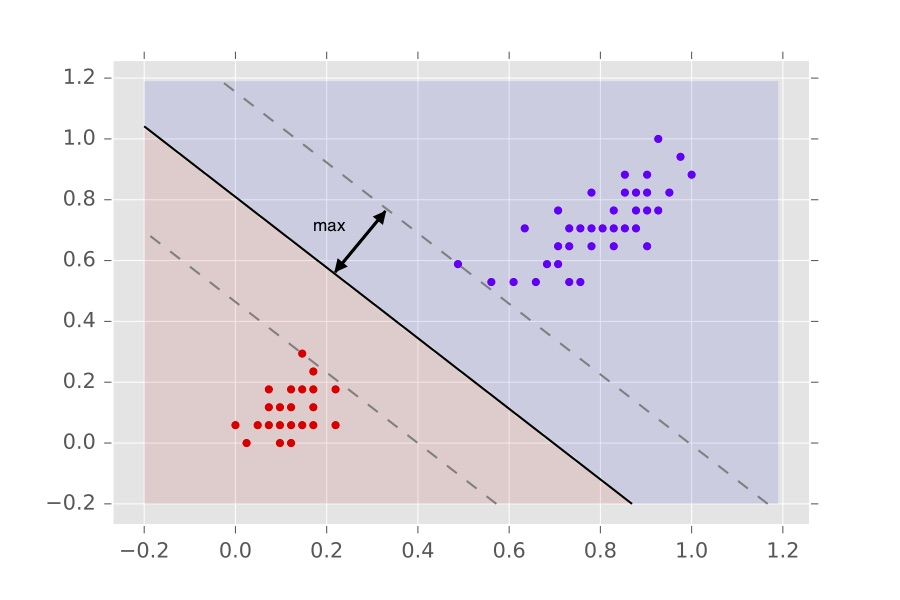
\includegraphics[width=0.7\textwidth]{slike/LinearnoLocljiviIskanjeHiperravnine.jpg}
	\caption{Iskanje hiperravnine.}
	\label{slikaIskanjeHiperravnine}
\end{figure}



Zgornje pogoje lahko prevedemo v optimizacijski problem. Prvi dve zahtevi pravita: 
$$y_i = 1 \implies w^Tx_i+ b > 0$$
$$y_i = -1 \implies  w^Tx_i+ b < 0,$$
kar lahko ekvivalentno prepišemo v: 
$$  y_i(w^Tx+ b)> 0.$$
Oglejmo si sedaj, kako je z maksimiziranjem minimalne oddaljenosti od hiperravnine. 

\begin{definicija}
	Funkcija $r(x) = w^Tx + b$ predstavlja \emph{predznačeno razdaljo} do ravnine $\Pi= (w, b)$. 
\end{definicija}

Iz linearne algebre vemo, da je razdalja med ravnino $\Pi$ in točko $x$ definirana kot $\frac{|w^Tx+ b|}{||w||}$. Izraz $|w^Tx+ b|$ predstavlja razdaljo, pomnoženo z $||w||$. Če izrazu odvzamemo še absolutne vrednosti, dobimo predznačeno razdaljo. 

Ideja, kako postaviti optimizacijski problem, je, da postavimo najbližjo točko razreda $\pr$ na predznačeno razdaljo $1$ do hiperravnine, najbližjo točko razreda $\nr$ pa na predznačeno razdaljo $-1$. Sedaj vzamemo poljubno točko $x_+$, za katero velja  $w^Tx_++ b = 1 $, in njej zrcalno točko $x_-$ glede na hiperravnino $\Pi$, za katero velja $w^Tx_-+ b = -1 $. Velja tudi $x_+ = x_- + r w$, kjer je $r$ skalar, za faktor katerega se moramo od točke $x_-$ premakniti v smeri normalnega vektorja, da pridemo do zrcalne točke $x_+$. Vstavimo to v prvo enakost in dobimo:
$$ w^T( x_- + r w)  + b = 1. $$
Iz linearnosti skalarnega produkta sledi: 
$$ w^Tx_-  + rw^Tw+ b = 1. $$
Prvi in zadnji člen se po definiciji $x_-$ seštejeta v $-1$, od koder sledi 
$$ r = \frac{2}{||w||}.$$
\begin{figure}[H]
	\centering
	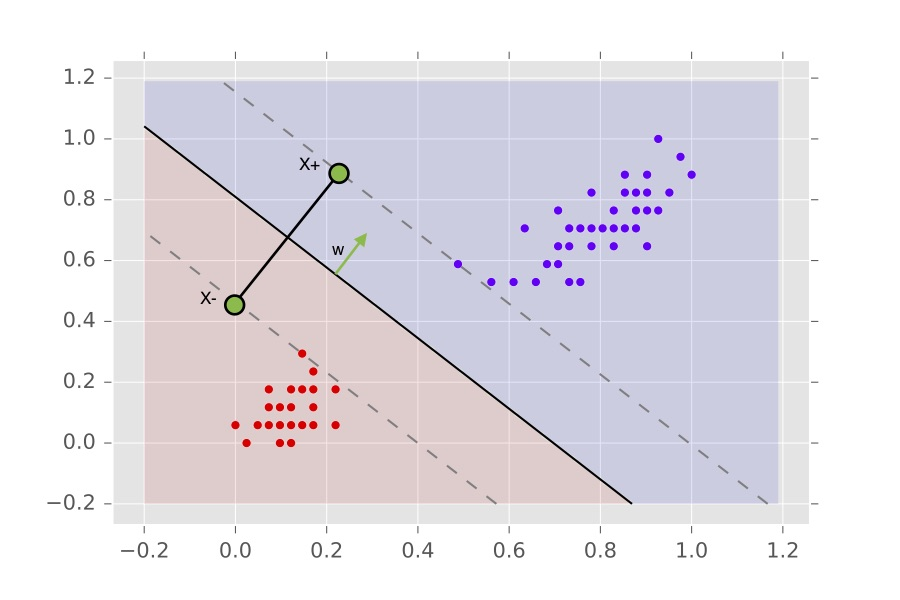
\includegraphics[width=0.7\textwidth]{slike/LinearnoLocljiviOptimizacija.jpg}
	\caption{Ideja minimizacijskega problema.}
	\label{slikaIdejaMinimizacijskegaProblema}
\end{figure}
Zadnja točka pogojev iskanja želene hiperravnine pove, da je naš problem maksimiziranje $r$, kar je ekvivalentno minimizaciji $||w||$ ali $||w||^2.$ Minimizirali bomo $||w||^2$, da se izognemo korenom. 
Če sta $(w, b)$ parametra neke hiperravnine, sta tudi $(\alpha w, \alpha b)$ parametra iste hiperravnine, zato lahko izbiramo med takimi $(w, b)$, kjer v minimumu dosežemo, da je $y_i(w^T+b) =1$ za vsaj en podatek, hkrati pa za vse preostale točke velja: $y_i(w^T+b) \ge 1.$
Zapišimo sedaj celoten minimizacijski problem: 
\begin{align}
\label{min_prvic}
\begin{split}
\min_{w \in \R^n, b \in \R}  &||w||^2  \\
\text{pri pogojih}~ &y_i(w^Tx_i + b)\ge 1,  ~ i= 1, 2, \ldots, m
\end{split}
\end{align}
\begin{definicija}
	Optimizacijski problem je \emph{dopusten}, če obstaja rešitev, ki ustreza vsem pogojem problema. 
\end{definicija}
Zgornji problem je dopusten, ker smo predpostavili, da so naši podatki linearno ločljivi. Množici točk, ki ustrezajo vsem pogojem optimizacijskega problema, pravimo množica \emph{dopustnih rešitev}. 
V rešitvi optimizacijskega problema bo vsaj en predstavnik razreda $\pr$ na predznačeni razdalji $1$ in vsaj en predstavnik razreda $\nr$ na predznačeni razdalji $-1$. Noben podatek pa ne bo po absolutni vrednosti bližje hiperravnini $(w, b)$.

\subsection{Omilitev linearne ločljivosti}\label{ssec:SplosniPodatki}
Sedaj se lotimo podatkov, ki v splošnem niso linearno ločljivi, torej ne obstaja hiperravnina, ki bi strogo ločila podatke. Radi bi dopolnili metodo iz prejšnjega razdelka do te mere, da bo še vedno delovala. Če poskusimo rešiti  minimizacijski problem \eqref{min_prvic}, ne dobimo nobene dopustne rešitve. Zato moramo omiliti pogoje, da bomo dobili dopusten optimizacijski problem. Pri prejšnjem problemu smo okrog hiperravnine ustvarili pas na predznačeni razdalji od $-1$ do $1$, v katerem ni bilo nobenega podatka. Sedaj bomo ta pogoj omili. 

Vsakemu podatku dovolimo, da lahko leži tudi znotraj omenjenega pasu, ali pa celo na nasprotni strani, vendar mora za to plačati določeno ceno, ki jo vnaprej postavimo. Podatku $x_i$ dodamo spremenljivko $e_i \in \R, e_i \ge 0$, ki pove, kako močno dani podatek krši naše zahteve. Omejitve popravimo v zgornjem duhu, tako da velja: 
\begin{align}
\label{PodV}y_i(w^Tx_i + b) &\ge 1 - e_i,  ~ i= 1, 2, \ldots, m \\
\nonumber e_i &\ge 0 , ~i = 1, \ldots, m
\end{align}
Iz teh pogojev tudi vidimo, kje natančno lahko leži točka. Če je $e_i = 0$, potem točka leži na pravi strani pasu, če je $0 \le e_i \le 2$ točka leži znotraj pasu, če pa je $e_i  > 2$, točka leži na napačni strani, zunaj pasu. 


Popravili bomo še funkcijo, ki jo minimiziramo. Dodali bomo faktor, s katerim reguliramo, kako močno kaznujemo podatek, ki ne leži na svoji strani pasu. Namesto minimuma $||w||^2$, bomo sedaj iskali minimum izraza $\frac{1}{2}||w||^2 + C\sum_{i = 1}^{m}e_i$. Celoten optimizacijski problem se glasi: 
\begin{align}
\label{NPP}
\begin{split}
\min_{w, b, e}~&\frac{1}{2}||w||^2 + C\sum_{i = 1}^{m}e_i \\
\text{p.p.} ~ &y_i(w^Tx_i + b)\ge 1 - e_i, ~i= 1, 2, \ldots, m\\
&e_i \ge 0, i = 1, \ldots, n
\end{split}
\end{align}
Tu je $C$ izbran nenegativen parameter, $e = (e_1, \ldots e_n)$ pa \emph{vektor odstopanja}. Izberimo si poljubna $w$ in $b$. S povečevanjem $e_i$ dobimo rešitev, ki je dopustna, torej je naš optimizacijski problem dopusten. Če je $e_i > 0$, potem je v $i$-ti omejitvi pri optimalni rešitvi dosežena enakost, saj bi v nasprotnem primeru obstajala strogo boljša rešitev. Točkam $x_i$, v katerih je dosežena enakost $y_i(w^Tx_i + b) = 1 - e_i$, pravimo \emph{podporni vektorji}. Njihov pomen bo prišel do izraza, ko se bomo ukvarjali z metodami jeder. 


 V praksi se zgornji optimizacijski problem uporablja tudi, če so podatki linearno ločljivi. Razlog tiči v \emph{preprileganju}. Moramo se zavedati, da je naš cilj še vedno najti čim boljši napovedni model za nove podatke. S tem namenom potem tudi pustimo nekaterim podatkom, da ne ležijo na pravi strani pasu, v upanju, da bo naš model zajel večjo splošnost. Če postavimo $C$ na neskončno, potem se zgornji optimizacijski problem prevede na problem z ločljivimi podatki. Čim manjši kot je $C$, tem bolj splošno sliko zajamemo, hkrati pa dobimo tudi več \emph{podpornih vektorjev}. Po drugi strani lahko s premajhnim $C$-jem povsem zgrešimo smer, kjer naj bi meja potekala. 

\subsection{Večrazredni podatki}
\label{poglavjeVecrazredniPodatki}
V tem razdelku se bomo srečali z metodami, s katerimi si pomagamo, če podatki ne pripadajo samo dvema razredoma, ampak poljubno mnogim. Predstavili bomo dve najpogostejši metodi. 
\subsubsection{Ena na ena}
Ena iz med teh metod je metoda ``Ena na ena''. Recimo, da imamo $N$ različnih razredov, katerim pripadajo podatki. Pri tej metodi vzamemo vse podatke, ki pripadajo $i$-temu in $j$-temu razredu, ter jih ločimo s standardnimi metodami za ločevanje dveh razredov, ki so opisane zgoraj. Tako dobimo $\binom{N}{2}$ različnih mej med razredi. Ko želimo napovedati, kateremu razredu pripada novi podatek, izvedemo glasovanje. To poteka tako, da gre podatek preko vseh $\binom{N}{2}$ napovednih modelov. Ko napovemo, ali podatek pripada razredu $i$ ali $j$, zmagovalni razred dobi glas (ponavadi enega, lahko pa moč glasu tudi utežimo s tem, kako prepričani smo, da podatek pripada temu razredu. Prepričanost ocenjujemo s tem, kako daleč stran od meje leži podatek.). Na koncu podatku določimo razred, za katerega je prejel največ glasov. 
\subsubsection{Eden proti vsem}\label{poglavjeEdenProtiVsem}
Pri tej metodi namesto $\binom{N}{2}$ klasifikatorjev določimo $N$ različnih funkciji, ki nam vrnejo predznačene razdalje. Tako funkcijo $i$ določimo tako, da $i$-ti razred predstavimo kot razred $\pr$, vse ostale podatke pa združimo v razred $\nr$. Nov podatek napovemo na naslednji način. Podatek izvrednotimo v vseh $N$ prej izračunanih funkcijah in mu določimo tisti razred, za katerega izračunane funkcije vrnejo največjo vrednost. Če je $i$-ta funkcija vrnila največjo vrednost, določimo, da podatek pripada $i$-temu razredu. 



\subsection{Nelinearni podatki}
\label{poglavjeNelinearniPodatki}
Mnogokrat imamo opravka s podatki, katere je nesmiselno ločevati s hiperravnino, ki pa jih lahko zelo enostavno ločimo s kakšno nelinearno hiperploskvijo. 
\begin{figure}[H]
	\centering
	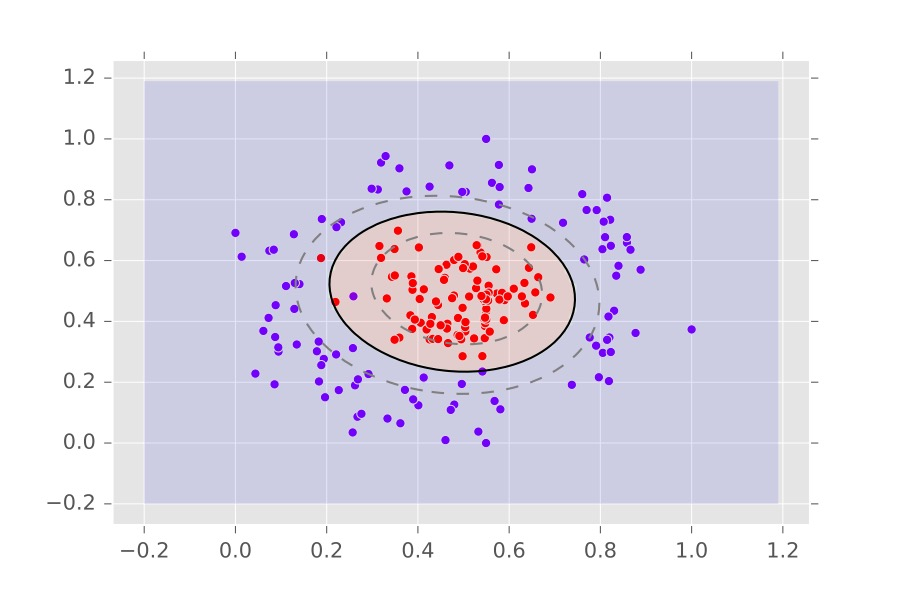
\includegraphics[width=0.7\textwidth]{slike/RadialniPodatkiPolinomskaMeja.jpg}
	\caption{Primer podatkov, ki jih ni smiselno ločevati s hiperravnino.}
	\label{slikaPrimerPodatkovKiJihNiSmiselnoLocevatiSHiperploskvijo}
\end{figure}
S takim problemom se spopademo tako, da prostor začetnih podatkov preslikamo v nov prostor (ponavadi višjih dimenzij). Nato podatke v preslikanem prostoru linearno ločimo. Ta novonastala meja se v prvotnem prostoru izraža kot nelinearnost (pogoj za nelinearnost je, da so funkcije začetnih podatkov, ki dodajo nove dimenzije, nelinearne). Oglejmo si primer, ko so začetni podatki v $\R^2$. Podatke $(x, y)$ bi razširili v $(x, y, x^2, y^2)$ ter nato poiskali mejo med njimi tako kot v \eqref{NPP}. Problem, kjer imamo $m$ takšnih podatkov, bi lahko opisali kot: 
\begin{align}
\nonumber\min_{w, b, e}~&\frac{1}{2}||w_1||^2 +\frac{1}{2}||w_2||^2 +  C\sum_{i = 1}^{m}e_i \\
\nonumber\text{p.p.} ~ &y_i(w_{11}x_i + w_{12}y_i + w_{21}x_i^2 + w_{22}y_i^2  + b)\ge 1 - e_i, ~i= 1, 2, \ldots, m\\
\nonumber&e_i \ge 0,~ i = 1, \ldots, m
\end{align}
Naslednja ideja bi bila, da da bi podatkom $(x, y)$ dodali še kakšen monom, sestavljen iz $x, y $, kot recimo $(x, y,xy, x^2, y^2, x^3y)$. Ustrezno bi morali popraviti tudi optimizacijski model. Tako bi lahko začetnim podatkom dodali poljubno število novih dimenzij, ki jih sestavimo kot monome začetnih podatkov. S tem bi določili neko polinomsko ločitveno hiperploskev. Tu naletimo na problem časovne zahtevnosti. Začetni prostor podatkov preslikamo v prostor z veliko večjo dimenzijo. Nastali optimizacijski problem postane precej zahtevnejši. Če bi želeli dobiti klasifikacijo poljubne hiperploskve, ki jo sestavimo iz začetnih podatkov $X \in \R^{m\times n}$ iz monomov največje stopnje $k$, bi se  začetni prostor za $w$ preslikal iz dimenzije $n$ v dimenzijo $\binom{n + k}{k}$, kjer smo upoštevali, da za monom štejemo tudi $1$. Problem z večanjem stopnje $k$ postane zelo hitro računsko prezahteven za računalnik. Na ta način pa za mejo sploh ne moremo dobiti funkcije, ki je neskončna vsota polinomov. Kaj mislimo s tem, bo jasneje v nadaljevanju. V želji, da nas dodajanje dimenzij in ločevanje z nelinearnimi hiperploskvami ne bi omejilo, bomo najprej v poglavju \ref{dual} spoznali nekaj teorije dualnih optimizacijskih problemov. V nadaljevanju bomo v poglavju \ref{updual} s pomočjo pridobljene teorije optimizacijski problem \eqref{NPP} prevedli na dualni problem, s pomočjo katerega bomo rešili zagato z računsko zahtevnostjo. 

\section{Dualnost}
\label{dual}

V tem poglavju bomo spoznali teorijo \emph{dualnih konveksnih problemov}. S pomočjo pridobljenega znanja bomo prevedli optimizacijski problem \eqref{NPP} na njegov \emph{dualni problem}, katerega optimalna vrednost je enaka optimalni vrednosti \emph{primarnega problema}. 

\subsection{Definicija dualnega problema}
V prvem poglavju smo se srečali z optimizacijsko nalogo, ki jo v splošnem lahko napišemo kot:
\begin{align}
\label{PP}f^* =  \min~ &f(x),\\ 
\nonumber	\text{p.p. } &g_i(x) \le 0, ~ i = 1,2,\ldots,m, \\
\nonumber	&h_j(x) = 0, ~j = 1, 2, \ldots,p, \\
\nonumber	&x\in X,
\end{align}
kjer so $f, g_i, h_j ~(i=1,2,\ldots,m,~ j=1, 2,\ldots p)$ funkcije, definirane na $X \subseteq \R^n$. Problem \eqref{PP} poimenujemo \emph{primarni problem}. Lagrangeeva funkcija za zgornji problem se glasi: 
\begin{align*}
L(x, \lambda, \mu) = f(x)+ \sum_{i=1}^{m}\lambda_ig_i(x) + \sum_{j=1}^{p}\mu_ih_j(x)\quad (x \in X, \lambda \in \R_+^m, \mu \in \R^p).
\end{align*}
Tukaj nenegativne Lagrangeeve množitelje $\lambda_i$ dobimo iz omejitev z neenakostmi, Lagrangeeve množitelje $\mu_j$ pa iz omejitev z enakostmi. \emph{Dualna funkcija} $q: \R_+^m \times \R^p \to \R \cup \{-\infty\}$ je definirana kot:
\begin{align*}
q(\lambda, \mu) = \inf_{x \in X}L(x, \lambda, \mu).
\end{align*} 
Lahko se tudi zgodi, da infimum ni končen -- obstajajo vrednosti $(\lambda, \mu)$, za katere je $q(\lambda, \mu)= - \infty$. Zato definiramo \emph{končno domeno} dualne funkcije: 
\begin{align*}
\dom(q) = \{(\lambda, \mu) \in \R_+^m \times \R^p: q(\lambda, \mu) > - \infty\}.
\end{align*}
\emph{Dualni problem} problema \eqref{PP} se glasi: 
\begin{align}
\label{DP} &q^* = \max q(\lambda, \mu)\\ 
\nonumber &\text{p.p.} ~ (\lambda,\mu) \in \dom(q). 
\end{align}

\begin{opomba}
	Kljub temu, da v primarnem in dualnem problemu iščemo minimum oz. maksimum, se lahko zgodi, da je problem neomejen. Striktno gledano bi morali uporabljati oznaki infimum oz. supremum, vendar bomo, zaradi standardne oznake, pisali minimum oz. maksimum.
\end{opomba}


Naslednja trditev nam bo pomagala dokazati izrek \ref{KD}, ki pravi, da je dualni problem konveksen problem. To pomeni, da minimiziramo konveksno (ali maksimiziramo konkavno) funkcijo na konveksnem območju. 

\begin{trditev} \label{sk}
	Naj bo $f_i: \R^n \to \R, i \in I$ družina konveksnih funkcij. Potem je tudi $f(x) = \sup_{i \in I}f_i(x)$ konveksna. 
\end{trditev}

\begin{dokaz}
	Izberimo poljuben $i\in I$ in $\alpha \in [0,1].$ Velja:
	\begin{align*}
	f_i(\alpha  x + (1-\alpha ) y) &\le \alpha  f_i(x)  + (1-\alpha ) f_i(y) \\
	& \le  \sup_{i' \in A} (\alpha  f_{i'}(x)  + (1-\alpha ) f_{i'}(y)) \\
	& \le  \sup_{i' \in A} \alpha  f_{i'}(x)  + (1-\alpha ) \sup_{i' \in A}f_{i'}(y) \\
	&= \alpha  f(x) + (1-\alpha ) f(y).
	\end{align*}
	Ker je bil $i$ poljuben, velja ta neenakost tudi za supremum. Dobimo:
	$$ f(\alpha  x + (1-\alpha ) y) \le \alpha  f(x) + (1-\alpha ) f(y),$$
	to pa ravno pomeni, da je $f$ konveksna. 
\end{dokaz}

\begin{posledica}
	\label{psk}
	Naj bo $f_i: \R^n \to \R, i \in I$ družina konkavnih funkcij. Potem je tudi $f(x) = \inf_{i \in I}f_i(x)$ konkavna. 
\end{posledica}

\begin{dokaz}
	Družina funkcij $-f_i\in I$ je konveksna, zato po izreku \ref{sk} sledi, da je funkcija $-f = \inf_{i \in I}(-f_i(x)) =  -\sup_{i \in I}f_i(x)$ konveksna funkcija. Torej je $f$ konkavna.
\end{dokaz}

\begin{izrek}[Konveksnost dualnega problema]\label{KD}
	Naj bo problem kot \eqref{PP} ter $f, g_i$ in $h_j~ (i = 1,2,\ldots,m, j=1,2,\ldots,p)$ omejene funkcije, definirane na množici $X \subseteq \R^n$. Naj bo $q$ dualna funkcija tega problema. Potem velja:
	\begin{enumerate}[(i)]
		\item 
		$\dom(q)$ je konveksna množica, 
		\item 
		$q$ je na $\dom(q)$ konkavna funkcija 
	\end{enumerate}
\end{izrek}

\begin{proof}
	Izberimo si poljubni točki $(\lambda_1, \mu_1), (\lambda_2, \mu_2) \in \dom(q)$ in $\alpha \in [0,1]$. Iz definicije $\dom(q)$ sledi: 
	\begin{align*}
	&\inf_{x \in X} L(x, \lambda_1, \mu_1) >- \infty\\
	&\inf_{x \in X} L(x, \lambda_2, \mu_2) >- \infty.
	\end{align*}
	Ker je Lagrangeeva funkcija $L(x, \lambda, \mu)$ afina glede na $\lambda$ in $\mu$, sledi: 
	\begin{align*}
	q(\alpha\lambda_1 + (1-\alpha)\lambda_2, \alpha\mu_1 + (1-\alpha)\mu_2) &= \inf_{x \in X}L(x,\alpha\lambda_1 + (1-\alpha)\lambda_2, \alpha\mu_1 + (1-\alpha)\mu_2 )\\
	&= \inf_{x \in X}\big(\alpha  L(x, \lambda_1, \mu_1) + (1-\alpha)L(x, \lambda_2, \mu_2) \big)\\
	&\ge \alpha \inf_{x \in X}L(x, \lambda_1, \mu_1) + (1-\alpha)\inf_{x \in X}L(x, \lambda_2, \mu_2)\\
	&=\alpha q(\lambda_1, \mu_1) + (1-\alpha)q(\lambda_2, \mu_2)\\
	&>-\infty.
	\end{align*}
	S tem smo dokazali konveksnost množice $\text{dom}(q).$
	
	Za vsak $x\in X$ in $(\lambda, \mu) \in \dom(q) $ je Lagrangeeva funkcija $L(x, \lambda, \mu)$ afina glede na $(\lambda, \mu)$, zato je tudi konkavna glede na $(\lambda, \mu)$. Ker je $q(\lambda, \mu)$ infimum konkavnih funkcij, je po posledici \ref{psk} konkavna. 
\end{proof}

Naslednji izrek pove, da je optimalna vrednost, ki jo dobimo pri reševanju dualnega problema, vedno manjša ali enaka rešitvi začetnega problema. 


\begin{izrek}[Šibki izrek o dualnosti]
	Naj bo $f^*$ optimalna vrednost primarnega problema \eqref{PP} in $q^*$ optimalna vrednost dualnega problema \eqref{DP}. Potem velja:
	$$ q^* \le f^*.$$
\end{izrek}

\begin{dokaz}
	Označimo množico dopustnih rešitev s $S:$
	$$ S = \{x \in X; g_i(x) \le 0, h_j(x) = 0, i = 1, \ldots, m, j = 1, \ldots, p \}.$$
	Za vsak $(\lambda, \mu) \in \R_+^m \times \R^p$ velja: 
	\begin{align*}
	q(\lambda, \mu) &= \inf_{x \in X} L (x, \lambda, \mu) \\
	&\le \inf_{x \in S} L (x, \lambda, \mu)\\
	&= \inf_{x \in S} \Big(f(x)  + \sum_{i=1}^{m}\lambda_ig_i(x) + \sum_{j=1}^{p}\mu_jh_j(x) \Big)\\
	&\le \inf_{x \in S} f(x) = f^*.
	\end{align*}
	V zgornjem izrazu zadnja neenakost velja, ker je za vsak $x \in S$ $h_j(x) = 0$ ter $\lambda_ig_i(x) \le 0$, saj je po definiciji $\lambda_i \ge 0$ ter $g_i(x) \le 0$  za vsak $x \in S.$ 
	Dokazali smo, da za vsak $(\lambda, \mu) \in \R_+^m \times \R^p$ velja $q(\lambda, \mu) \le f^*$. Zato zgornja neenakost velja tudi za maksimalno vrednost. 
\end{dokaz}

\subsection{Krepka dualnost v primeru konveksnega problema}
V splošnem ni vedno res, da je vrednost dualnega problem enaka vrednosti primarnega problema. Oglejmo si primer, kjer ne dosežemo enakosti.
\begin{primer}
	Rešimo optimizacijsko nalogo: 
	\begin{align*}
	& \min x^2 - 3y^2 \\
	& ~\text{p.p.} ~ x=y^3, x, y\in \R 
	\end{align*}
	Namesto $x$ vstavimo $y^3$. Dobimo:
	\begin{align*}
	& \min y^6 - 3y^2 \\
	\end{align*}
	Ker je minimizacijska funkcija polinom sode stopnje s pozitivnim vodilnim koeficientom, bo minimum dosežen v stacionarni točki.  Stacionarne točke so rešitve enačbe:
	\begin{align*}
	6y^5 -6y = 6y(y^4 -1) = 0.
	\end{align*}
	Edini kandidati za optimalno rešitev $(x, y) $ so torej $(0,0), (1,1), (-1,-1)$. Ko to vstavimo v minimizacijsko funkcijo, dobimo rešitev optimizacijske naloge $f^*=-2.$ Sedaj pa si oglejmo dualni problem zgornjega problema. Lagrangeeva funkcija se glasi:
	\begin{align*}
	L(x, y, \mu) = x^2 -3 y^2 + \mu(x-y^3) = x^2 + \mu x -3y^2 - \mu y^3
	\end{align*}
	Za vsak $\mu$ velja:
	\begin{align*}
	\inf_{x, y}L(x,y,\mu) = -\infty.
	\end{align*}
	Torej dualni problem sploh nima dopustnih rešitev, oz. v bolj ohlapnem smislu ima vrednost $-\infty$, kar je zelo slaba ocena za vrednost primarnega problema $f^* = -2.$
\end{primer}

Enakost velja, ko imamo opravka s konveksnim območjem in konveksno funkcijo, kot je tudi naša ciljna funkcija, za katero gradimo teorijo. 
Sedaj si oglejmo nekaj lem in trditev, ki nam bodo pomagale dokazati izrek o separaciji dveh konveksnih množic. S slednjim izrekom si bomo pomagali pri dokazu nelinearne Farkaseve leme. Ta bo ključna pri dokazu, da v konveksnem primeru primarni in dualni problem dosežeta enako optimalno vrednost. 


\begin{trditev}\label{podpornik}
	Naj bo $C$ neprazna, zaprta in konveksna podmnožica v $\R^n$. Naj bo $x_0 \in \R^n$ točka, ki ne leži v $C$. Potem obstajata taka $a_0 \in C$ in $0\ne p \in \R^n$, da za vsak $a \in C$ velja:
	$$p^T x_0 < p^Ta_0 \le p^Ta.  $$
\end{trditev}

\begin{dokaz}
	Ker je množica $C$ neprazna, obstaja točka $z\in C$. Sedaj vpeljimo oznako $Z = C \cap \Cl(K(x_0, ||z-x_0||))$. Ker je $Z$ zaprta in omejena,  je kompaktna. Funkcija $d(x) = ||x-x_0||$ je zvezna, zato doseže na $Z$ minimum. Označimo z $a_0$ točko, kjer funkcija $d$ doseže minimum. Po konstrukciji za točke v $C \cap Z^C$ velja, da so kvečjemu bolj oddaljene od $x_0$ kot vse točke v $Z$. Torej je v $a_0$ dosežen tudi globalni minimum na $C$. Označimo $p = a_0 - x_0.$ Ker $x_0 \notin C$, je $p \ne 0.$Velja: 
	\begin{align*}
	p^Tx_0 &= p^T(x_0 - a_0) + p^Ta_0\\
	&= -||p||^2 + p^Ta_0 \\
	&< p^Ta_0.
	\end{align*}
	
	
	Sedaj pokažimo, da za vsak $a\in C$ velja $p^Ta_0 \le p^Ta$. Ker je množica $C$ konveksna, je za vsak  $t \in [0,1]$ $w := a_0 + t(a-a_0)  \in C$. Velja:
	\begin{align*}
	||x_0 - a_0||^2  - ||x_0 - w||^2  &= (x_0 - a_0)^T(x_0 - a_0) -\\
	& (x_0 - a_0 + t(a_0-a))^T(x_0 - a_0 + t(a_0-a))\\
	&= -2t(a_0 - a)^T(x_0 - a) - t^2(a_0 - a)^T(a_0 - a) \\
	&= t (2p^T(a_0-a) - t||a_0-a||^2).
	\end{align*}
	Po konstrukciji točke $a_0$ je zgornji izraz vedno manjši ali enak $0$. Zato za vsak $t \in (0,1]$ velja
	\begin{align*}
	2p^T (a_0 - a )- t ||a_0-a|| \le 0.
	\end{align*}
	Sedaj pošljemo $t$ proti 0 in dobimo 
	\begin{align*}
	2p^T(a_0-a) \le  0,
	\end{align*}
	kar lahko zapišemo kot $p^Ta_0 \le p^Ta$.
\end{dokaz}

\begin{lema}\label{konveksnozaprtje}
	Naj bo $C \subseteq \R^n$ konveksna množica. Potem je tudi $\Cl(C)$ konveksna.
\end{lema}

\begin{dokaz}
	Izberimo si $x, y \in \Cl(C)$ in $\lambda \in [0,1]$. Ker je $\Cl(C)$ zaprta, obstajata zaporedji $\{x_k\}_{k\ge0} \subseteq C$ in $\{y_k\}_{k\ge0} \subseteq C$, ki zaporedoma limitirata proti $x$ in $y$. Ker je $C$ konveksna, sledi, da za vsak $k \ge 0$ velja $\lambda x_k + (1 - \lambda )y_k \in C$. Zaporedje $\lambda x_k + (1 - \lambda )y_k$ konvergira proti   $\lambda x + (1 - \lambda )y$. Torej obstaja zaporedje v $C$, ki konvergira proti $\lambda x + (1 - \lambda )y$. Torej je  $\lambda x + (1 - \lambda )y \in \Cl(C)$.
\end{dokaz}


\begin{lema}\label{sp}
	Naj bosta $x \in \Int(C)$ in $y \in \Cl(C)$, kjer je $C$ konveksna množica z neprazno notranjostjo. Potem je $(1-\lambda)x + \lambda y \in \Int(C) $za vsak $\lambda \in (0,1).$
\end{lema}

\begin{dokaz}
	Ker je $x \in \Int(C)$, obstaja tak $\epsilon > 0$, da velja $K(x, \epsilon) \subseteq C$. Naj bo $z = (1-\lambda)x + \lambda y$. Dokazali bomo, da je $K(z, (1-\lambda)\epsilon) \subseteq C$. Izberimo poljuben $w$, ki zadošča $||w-z|| < (1-\lambda)\epsilon$. Ker je $y\in \Cl(C)$, vsaka krogla s središčem v $y$ seka $C$. Izberimo si tak $w_1$, ki je vsebovan v preseku $C \cap K(y, \frac{(1-\lambda)\epsilon-||w-z||}{\lambda})$. Za ta $w_1 \in C$ torej velja:
	$$ ||w_1 - y|| < \frac{(1-\lambda)\epsilon - ||w-z||}{\lambda}.$$
	Naj bo $w_2 = \frac{1}{1-\lambda}(w - \lambda w_1)$. Potem velja: 
	\begin{align*}
	||w_2 -x|| &= \bigg|\bigg|\frac{w-\lambda w_1}{1-\lambda} - x\bigg|\bigg| \\
	&=\frac{1}{1-\lambda}||(w-z) + \lambda(y - w_1)|| \\
	&\le \frac{1}{1-\lambda}(||w-z|| + \lambda||w_1 - y||) \\
	&< \epsilon.
	\end{align*}
	Torej je $w_2 \in C$. Ker je $w = \lambda w_1 + (1-\lambda)w_2$ in je $C$ konveksna, je tudi $w \in C$. Ker je $K(z, (1-\lambda)\epsilon) \subseteq C$, je $z \in \Int(C).$
\end{dokaz}




\begin{lema}
	Naj bo $C \subseteq \R^n$ konveksna množica z neprazno notranjostjo. Potem velja: 
	$$ \Int(\Cl(C)) = \Int(C).$$
\end{lema}

\begin{dokaz}
	Ker velja $C \subseteq \Cl(C)$ sledi $\Int(C) \subseteq \Int (\Cl(C))$. 
	
	
	Dokažimo sedaj še obratno vsebovanost. Naj bo $x \in \Int(\Cl(C))$ poljuben. Ker je $x \in \Int(\Cl(C))$, obstaja tak $\epsilon > 0$, da je $K(x, \epsilon) \subseteq \Cl(C)$. Vzemimo sedaj $y \in \Int(C)$. Če je $y = x$, je seveda tudi $ x \in \Int(C)$. Sicer definirajmo $z = x + \alpha(x - y)$, kjer je $\alpha = \frac{\epsilon}{2||x-y||}$. Ker je $||z-x|| = \frac{\epsilon}{2}$, je $z \in \Cl(C)$. Torej je po lemi \ref{sp} $(1-\lambda)y + \lambda z \in \Int(C)$ za  vsak $\lambda \in (0,1)$. V posebnem je to res tudi za $\lambda_\alpha = \frac{1}{1+\alpha} \in (0,1)$. Če iz enakosti $z = x + \alpha(x - y)$ izrazimo $x$ dobimo 
	\begin{align*}
	x &= \frac{\alpha}{1+\alpha}y +\frac{1}{1+\alpha} z\\
	&= (1-\lambda_{\alpha})y + \lambda_{\alpha}z.
	\end{align*}
	Torej je $x \in \Int(C)$.   
\end{dokaz}



\begin{izrek}[O podporni hiperravnini]
	Naj bo $C\subseteq \R^n$ konveksna množica in naj bo $y \notin C$. Potem obstaja tak $0 \ne p \in \R^n$, da za vsak $x \in C$ velja:
	$$ p^Tx \le p^Ty.$$
\end{izrek}

\begin{dokaz}
	Ker $y \notin \Int(C)$, sledi, da $y \notin \Int(\Cl(C))$. 
	Torej obstaja zaporedje $ \{y_k\}_{k\ge 1}$, za katero velja $y_k \notin \Cl(C)$ ter $\lim_{k \to \infty} y_k = y$. $\Cl(C)$ je konveksna po lemi \ref{konveksnozaprtje}
	ter zaprta po definiciji, zato iz trditve \ref{podpornik} sledi, da za vsak $k$ obstaja tak $0 \ne p_k \in \R^n$, da velja:
	$$ p_k^Tx < p_k^Ty_k$$ 
	za vsak $x \in \Cl(C)$. Sedaj delimo zadnjo neenakost s $||p_k||$ in dobimo: 
	\begin{align}\label{ne1}
	\frac{p_k^T}{||p_k||}(x-y_k)<0
	\end{align}
	za vsak $x \in \Cl(C)$. Ker je zaporedje $\{ \frac{p_k}{||p_k||}  \}_{k\ge1}$ omejeno, obstaja podzaporedje  $\{ \frac{p_k}{||p_k||}  \}_{k \in T}$, tako da velja:
	$$ \lim_{\substack{k \to \infty \\ k \in T}} \frac{p_k}{||p_k||} = p \in \R^n.$$
	Očitno je $||p|| = 1$. Ko pošljemo $k$ proti neskončnosti, dobimo iz neenakosti \eqref{ne1} neenakost: 
	$$ p^T(x-y) \le 0 $$
	za vsak $x \in \Cl(C)$. Ker je $C \subseteq \Cl(C)$, smo s tem dokazali izrek.  
\end{dokaz}

\begin{lema}\label{linkonv}
	Naj bodo $C_1$ in $C_2$ konveksni množici ter $\lambda_1, \lambda_2 \in \R$ poljubna skalarja. Potem je tudi $\lambda_1C_1 + \lambda_2 C_2$, definirana kot $\lambda_1C_1 + \lambda_2 C_2 = \{\lambda_1x_1 + \lambda_2x_2; x_1\in C_1, x_2 \in C_2	\},$ konveksna.  
\end{lema}

\begin{dokaz}
	Označimo  $x = \lambda_1 a_1 + \lambda_2 b_1$ in $y = \lambda_1 a_2 + \lambda_2 b_2$. Radi bi videli, da je $(1-\lambda)x + \lambda y \in \lambda_1C_1 + \lambda_2 C_2 $ za $\lambda \in [0,1]$. Velja: 
	$$(1-\lambda) (\lambda_1 a_1 + \lambda_2 b_1) + \lambda (\lambda_1 a_2 + \lambda_2 b_2) = \lambda_1((1-\lambda)a_1 + \lambda a_2) + \lambda_2((1-\lambda)b_1 + \lambda b_2). $$
	Ker je $C_1 $ konveksna, je $(1-\lambda)a_1 + \lambda a_2 \in C_1$. Iz enakega razloga je $(1-\lambda)b_1 + \lambda b_2 \in C_2$. Torej je $\lambda_1((1-\lambda)a_1 + \lambda a_2) + \lambda_2((1-\lambda)b_1 + \lambda b_2) \in  \lambda_1C_1 + \lambda_2 C_2$.
\end{dokaz}


\begin{izrek}[Separacija dveh konveksnih množic]
	Naj bosta $C_1, C_2\subseteq \R^n$ dve neprazni disjunktni konveksni množici. Potem obstaja tak $0 \ne p \in \R^n$, da za vsak $x \in C_1$ in vsak $y \in C_2$ velja: 
	$$ p^Tx\le p^Ty.$$
\end{izrek}


\begin{dokaz}
	Če v lemi \ref{linkonv} nastavimo vrednosti $\lambda_1 = 1$ in $\lambda_2 = -1$ vidimo, da je $C_1 - C_2$  konveksna. Ker je $C_1 \cap C_2 = \emptyset$, velja $0 \notin C_1 - C_2$. Po izreku o podporni hiperravnini zato obstaja $0 \ne p \in \R^n$, tako da velja:
	$$\forall x \in C_1, \forall y \in C_2: \quad p^T(x-y) \le p^T0 = 0.  $$
	To pa je ekvivalentno: 
	\begin{align*}
			\forall x \in C_1, \forall y \in C_2: \quad  p^Tx\le p^Ty. &\qedhere
	\end{align*} 
\end{dokaz}

Sedaj imamo vse pripravljeno, da dokažemo nelinearno Farkasevo lemo. Ta bo ključnega pomena pri dokazu, da je pri določenih predpostavkah rešitev dualnega problema enaka rešitvi primarnega problema. 

\begin{izrek}[Nelinearna Farkaseva lema]
	Naj bo $X \subseteq \R^n$ konveksna množica in naj bodo $f, g_1, \ldots, g_m$ konveksne funkcije na $X$. Naj obstaja točka $x_1 \in X$, za katero velja: 
	$$ g_1(x_1) < 0, \ldots, g_m(x_1) < 0. $$ 
	Naj bo $c \in \R$. Naslednji trditvi sta ekvivalentni: 
	\begin{enumerate}[(i)]
		\item 
		Drži implikacija
		$$x\in X, g_i(x) \le 0, i = 1,2, \ldots, m \implies   f(x) \ge c .$$
		\item 
		Obstajajo taki $\lambda_1, \ldots, \lambda_m \ge 0$, da velja
		\begin{align}
		\label{F2} \inf_{x \in X} \Big(f(x) + \sum_{i=1}^{m}\lambda_ig_i(x)\Big) \ge c.
		\end{align}
		
	\end{enumerate}
\end{izrek}

\begin{dokaz}
	Dokažimo najprej, da iz $(ii)$ sledi $(i).$ Recimo, da obstajajo $\lambda_1, \ldots, \lambda_m \ge 0$, tako da velja neenakost \eqref{F2}. Izberimo poljuben $x \in X$, za katerega za vse $i = 1,\ldots, m$ velja $g_i(x) \le 0$. Po predpostavkah je: 
	$$ f(x) + \sum_{i=1}^{m}\lambda_ig_i(x) \ge c.$$ 
	Ker velja $g_i(x) \le 0$ in $\lambda_i \ge 0$ sledi: 
	$$ f(x) \ge c  - \sum_{i=1}^{m}\lambda_ig_i(x)\ge c. $$
	
	
	Za dokaz v drugo smer pa se moramo malo bolj potruditi.
	Oglejmo si dve množici: 
	\begin{align*}
	S &= \{u = (u_0,\ldots, u_m); \exists x \in X, f(x) \le u_0, g_i(x) \le u_i, i = 1,2, \ldots, m				\}\\ 
	T &= \{(u_0,\ldots, u_m); u_0 < c, u_1 \le 0, \ldots, u_m\le 0				\}     
	\end{align*}
	Zaradi lastnosti točke $x_1$, je $(f(x_1), 0, \ldots, 0) \in S$. Točka $(c-1, 0,\ldots ,0)$ je v $T$. Torej sta $S$ in $T$ neprazni. 
	Trdimo, da sta $S$ in $T$ konveksni. Izberimo si $u = (u_0, \ldots, u_m) \in T$ in $v = (v_0,  \ldots, v_m) \in T.$ Za vsak $\lambda \in [0,1]$ velja:
	\begin{align*}
	(1-\lambda)u_0 + \lambda v_0 &< 	(1-\lambda)c + \lambda c = c \\
	(1-\lambda)u_i + \lambda v_i &\le 	(1-\lambda)0 + \lambda 0 = 0, ~ i = 1, \ldots, m.
	\end{align*}
	Torej je $T$ konveksna. Sedaj izberimo poljuben $u = (u_0, \ldots, u_m) \in S$ in poljuben $v = (v_0,  \ldots, v_m) \in S.$ Po definiciji množice $S$ obstajata točki $x$ in $y$, da velja: $f(x) \le u_0, g_i(x) \le u_i, ~ i=1, \ldots, m$ in $f(y) \le v_0, g_i(y) \le v_i, ~ i=1, \ldots, m$. Izberimo $\lambda \in [0,1]$. Ker je $X$ konveksna, je $(1-\lambda)x + \lambda y \in X.$ Hkrati pa zaradi konveksnosti funkcij $f$ in $g_i$, $i=1,\ldots, m$ velja:
	\begin{align*}
	&f((1-\lambda)x + \lambda y) \le (1-\lambda)f(x) + \lambda f(y) \le 	 (1-\lambda)u_0 + \lambda v_0	\\
	&g_i((1-\lambda)x + \lambda y) \le (1-\lambda)g_i(x) + \lambda g_i(y) \le 	 (1-\lambda)u_i + \lambda v_i, ~i=1,\ldots,m	
	\end{align*}
	Torej je $(1-\lambda)u + \lambda v \in S$ za vsak $\lambda \in [0,1]$. Posledično je $S$ konveksna.
	
	
	Sedaj bomo pokazali, da je presek množic $S$ in $T$ prazna množica. Vzemimo poljubno točko $u=(u_0, \ldots, u_m) \in S$. Po definiciji množice $S$ obstaja tak $x \in X$, da velja: $f(x) \le u_0, g_i(x) \le u_i$ za $i=1,\ldots, m$. Če obstaja $i \in {1,\ldots, m}$, tako da je $u_i  > 0$, potem $u \notin T$, saj $i$-ta komponenta ne zadošča definiciji množice $T$. Preveriti moramo samo še primer, ko velja $u_i \le 0, i = 1, \ldots, m$. Tedaj po $(i)$ velja, da je $c \le f(x)$. Ker velja tudi $f(x) \le u_0$, je $c \le u_0$. Torej $u \notin T$, ker $0$-ta komponenta ne ustreza definiciji množice $T$. Torej res velja $S \cap T = \emptyset.$  
	
	
	Po izreku o separaciji konveksnih množic sledi, da obstaja $a = (a_0, a_1, \ldots, a_m)\ne 0$, za katerega velja: 
	\begin{align*}
	\sum_{j=0}^{m}a_ju_j \ge\sum_{j=0}^{m}a_jv_j
	\end{align*}
	za vsak $u = (u_0, \ldots, u_m) \in S$ in $v = (v_0, \ldots, v_m) \in T$. V posebnem to velja tudi za:
	\begin{align}
	\inf_{u \in S}\sum_{j=0}^{m}a_ju_j \ge \sup_{u \in T}\sum_{j=0}^{m}a_ju_j. \label{nf1}
	\end{align}
	Sedaj bomo pokazali, da velja $a_i \ge 0$ za $ i = 0,1, \ldots, m$. Recimo, da bi za neki $i$ veljalo $a_i < 0$. Sedaj manjšamo $u_i$ na desni strani neenakosti \eqref{nf1}, tako da gre proti $-\infty$. Vse ostale komponente pustimo fiksne. Po definiciji množice $T$ ostanemo znotraj množice $T$. Supremum na desni strani enačbe \eqref{nf1} je poljubno velik, kar nas privede v protislovje.  
	
	Ker je $a \ge 0$, za $u = (u_0, \ldots, u_m) \in T$, kjer je $u_i \le 0$ in $a_i \ge 0$, velja $u_ia_i \le 0$ za $i=1,\ldots,m.$ Ker je $u_0 \le c$ in $a_0 \ge 0$ sledi:
	\begin{align*}
	\sum_{j=0}^{m}a_ju_j \le a_0c. 
	\end{align*}
	Ker se lahko vrednosti $a_0c$ na desni strani neenakosti \eqref{nf1} poljubno približamo, velja:
	\begin{align}
	\inf_{u \in S}\sum_{j=0}^{m}a_ju_j \ge a_0c. \label{nf2}
	\end{align}
	Sedaj bomo pokazali, da je $a_0 > 0$. Recimo, da bi vejalo, da je $a_0 =0$. Neenakost \eqref{nf2} se potem poenostavi v: 
	$$ \inf_{u \in S}\sum_{j=1}^{m}a_ju_j \ge 0. $$
	Sedaj uporabimo točko $x_1$ iz formulacije izreka. Ker velja $g_i(x_1) < 0$, si lahko izberemo $u_i = g_i(x_1)$ za $i = 1, \ldots m$, $u_0$ pa naj bo $f(x_1)$. Potem je točka $(u_0, \ldots,u_m)$ element $S.$ Dobimo: 
	$$ \sum_{j= 1}^{m}a_jg_j(x_1) \ge 0. $$
	Ker velja $a \ne 0$, mora obstajati vsaj ena komponenta $a_i$, ki je različna od $0$. S tem smo prišli v protislovje, saj je $g_i(x_1) <0$ in $a_i \ge 0$, za $i= 1, \ldots, m.$ Sledi, da je $a_0 > 0$.
	
	Neenačbo \eqref{nf2} sedaj delimo z $a_0$, ter vzamemo prvi člen iz vsote, tako da dobimo: 
	\begin{align}
	\inf_{u \in S} \Big( u_0 + \sum_{j=1}^{m}\widehat{a}_ju_j			\Big) \ge c,  \label{nf3}
	\end{align}
	kjer je $\widehat{a}_j = \frac{a_j}{a_0}$. Definiramo
	$$ \widehat{S} = \{u \in \R^{m+1}; \exists x \in X, \text{tako da: } f(x) = u_0, g_i(x) = u_i, i=1, \ldots, m \}.$$
	Velja $\widehat{S} \subseteq S.$ Od tu sledi:
	\begin{align*}
	c \le \inf_{u \in S} \Big( u_0 + \sum_{j=1}^{m}\widehat{a}_ju_j \Big)	&\le\inf_{u \in \widehat{S}} \Big( u_0 + \sum_{j=1}^{m}\widehat{a}_ju_j \Big)	\\
	&= \inf_{x \in X}\Big(f(x) + \sum_{j=1}^{m}\widehat{a}_jg_j(x)			\Big).
	\end{align*}	
	Če definiramo $\lambda_i = \widehat{a}_i$, vidimo, da smo pokazali, da iz $(i)$ sledi $(ii)$.
\end{dokaz}

Sedaj pa formulirajmo in dokažimo ključni izrek tega poglavja. Z njegovo uporabo bomo prevedli optimizacijski problem \eqref{NPP} na njegov dual. Z uporabo duala bomo naš prvotni problem lahko tudi posplošili.

\begin{izrek}[Krepki izrek o dualnosti za konveksne funkcije, omejitve podane z neenakostmi]\label{izrekdual}
	Naj bo
	\begin{align*}
	f^* =  \min f(x)\\ 
	\text{pri pogojih: } &g_i(x) \le 0, \quad i = 1,2,\ldots,m, \\
	&x\in X,
	\end{align*}
	kjer je $X$ konveksna množica in so $f, g_i, i = 1,\ldots,m$ konveksne funkcije na $X$, optimizacijski problem. Recimo, da obstaja točka $x_1 \in X$, za katero velja $g_i(x_1) < 0, i =1, \ldots, m$. Naj ima zgornji problem končno optimalno vrednost. Potem je optimalna vrednost dualnega problema
	$$  q^* = \max\{q(\lambda); \lambda \in \dom(q)\} $$
	kjer je 
	$$ q(\lambda) = \inf_{x\in X} L(x, \lambda) = \inf_{x \in X}\Big( f(x) + \sum_{i=1}^{m}\lambda_ig_i(x)	\Big)$$
	dosežena in velja, da sta optimalni vrednosti primarnega in dualnega problema enaki: 
	$$ f^* = q^*.$$	
\end{izrek}

\begin{dokaz}
	Ker je po predpostavkah  $f^* > -\infty$, velja: 
	$$ x\in X, g_i(x) \le 0, i = 1, \ldots, m \implies f(x) \ge f^*.$$
	Nelinearna Farkaseva lema pove, da obstajajo taki $\lambda_1, \ldots,  \lambda_m$, da velja: 
	$$ q(\lambda) = \inf_{x \in X} \Big(f(x) + \sum_{j=1}^{m}\lambda_jg_j(x)\Big)  \ge f^*.$$ 
	Sedaj uporabimo še šibki izrek o dualnosti in dobimo: 
	$$ q^* \ge q(\lambda) \ge f^* \ge q^*,$$
	torej velja $f^* = q^*$. Dodatno dobimo, da je $\lambda$ tudi optimalna rešitev dualnega problema. 
\end{dokaz}

\section{Uporaba dualnosti}
\label{updual}

\subsection{Prehod na dualni problem}

V tem poglavju bomo optimizacijski problem \eqref{NPP}  prevedli na njegov dualni problem.  
Razlog leži v tem, da dualni problem omogoča lažje reševanje in opis problemov, ko želimo podatke ločiti z nelinearno hiperploskvijo.  
Minimizacijski problem
\begin{align*}
\min{} &\frac{1}{2}||w||^2 + C\sum_{i = 1}^{m}e_i \\ 
\text{p.p. } &y_i( w^T x_i + b)\ge 1 - e_i,  \quad i= 1, 2, \ldots, m \\
&e_i \ge 0, \quad i = 1, \ldots, m \\
\end{align*}
najprej zapišimo v bolj kompaktni obliki: 
\begin{align*}
\min{} &\frac{1}{2}||w||^2 + C \mathds{1}^Te \\ 
\text{p.p. } &Y( Xw + b \mathds{1})\ge \mathds{1} - e,  \\
&e \ge 0, \\
\end{align*}
kjer so $Y = \diag(y_1, \ldots, y_m)\in \R^{m\times m}$, $\mathds{1} \in \R^m$ vektor enic, $X \in \R^{m\times n}$ matrika z vrsticami $x_1^T, \ldots, x_m^T$. 
Sedaj bomo ta problem zapisali v obliki, ki jo podaja izrek \ref{izrekdual}. Minimizacijska funkcija bo 
\begin{align*}
f^* = \min f(w, b, e) = \min \frac{1}{2}||w||^2 + C \mathds{1}^Te.
\end{align*}
Omejitvena funkcija $g_i$ bo $i$-ta vrstica neenakosti:
\begin{align*}
\mathds{1} - e - Y( Xw + b \mathds{1}) \le 0.
\end{align*}
Konveksno območje $X$, na katerem iščemo minimum, pa bo
\begin{align*}
X = \R^n \times \R \times (\R_+ \cup \{0\})^m,
\end{align*}
kjer so $w\in \R^n$, $b \in \R$ in $e \in  \R^m_+ \cup \{0\}.$ S tem smo s samo izbiro območja zadostili pogoju $e \ge 0$. Da bomo lahko uporabili izrek \ref{izrekdual}, moramo še pokazati, da so funkcije $f, g_i$ konveksne na $X$, da obstaja točka $(\widehat{w}, \widehat{b}, \widehat{e}) \in X$, za katero velja $g_i(\widehat{w}, \widehat{b}, \widehat{e}) < 0, i = 1, \ldots, m$, ter da ima naš problem končno optimalno vrednost.  Ker je optimizacijska funkcija $f$ vsota kvadratov $\frac{1}{2}w_i^2$ ter vsota linearnih členov $Ce_i$, ki so vse konveksne funkcije, je tudi $f$ konveksna.  Ker so vse omejitvene funkcije $g_i$ afine, so  posledično tudi konveksne. Sedaj bomo skonstruirali točko $(\widehat{w}, \widehat{b}, \widehat{e}) \in X$, za katero velja $g_i(\widehat{w}, \widehat{b}, \widehat{e}) < 0$ za vse $i = 1, \ldots, m$. Izberimo si poljubna $\widehat{w}$ in $\widehat{b}$. Za $\widehat{e_i}$ si izberemo: 
\begin{align*}
\widehat{e_i} = 
\begin{cases}
2 - y_i(\widehat{w}^Tx_i+\widehat{b});  &2 - y_i(\widehat{w}^Tx_i+\widehat{b}) \ge 0, \\
0;  &\text{sicer.}
\end{cases}
\end{align*}
Iz konstrukcije sledi, da za vsak $i$ velja: $g_i(\widehat{w}, \widehat{b}, \widehat{e}) < 0.$ Minimizacijska funkcija je navzdol omejena z $0$, saj je $e\ge 0$, $C\ge 0$, norma pa je vedno nenegativna. Ker je minimizacijski problem dopusten $((\widehat{w}, \widehat{b}, \widehat{e}) \in X)$ in navzdol omejen z $0$, ima končno optimalno vrednost. Sedaj lahko uporabimo izrek \ref{izrekdual} ter naš prvotni problem prevedemo na dualni, ki ima enako optimalno rešitev. Namesto črke $\lambda$ v izreku bomo tu uporabljali $\alpha \in \R^m.$  Zapišimo najprej Lagrangeevo funkcijo: 
\begin{align*}
L(w, b, e, \alpha) &= \frac{1}{2}||w||^2 + C\mathds{1} ^Te - \alpha^T(YXw + bY\mathds{1} -  \mathds{1}  + e) \\
&= \frac{1}{2}||w||^2 - w^TX^TY\alpha - b\alpha^TY\mathds{1}  + e^T(C\mathds{1} -\alpha) + \alpha^T\mathds{1} 
\end{align*}
Opazimo, da v Lagrangeevi funkciji členi z $w, b$ in $e$ nastopajo ločeno, torej lahko pošiščemo infimum vsakega posebej. 
\begin{align*}
q(\alpha) = \inf_{w}\bigg(\frac{1}{2}||w||^2 - w^TX^TY\alpha\bigg) + \inf_{b}\bigg(\!-b\alpha^TY\mathds{1}\!\bigg) + \inf_{e \ge 0}\bigg(\!e^T(C\mathds{1}-\alpha)\!\bigg) + \alpha^T\mathds{1}
\end{align*}
Oglejmo si sedaj, kaj so posamezni infimumi. Zadnja dva sta: 
\begin{align}
\nonumber\inf_{b}\bigg(-b\alpha^TY\mathds{1}\bigg) &= 
\begin{cases}
0; &\alpha^TY\mathds{1} = 0,\\
- \infty;  &\text{sicer,}
\end{cases}\\
\label{sndmin}\inf_{e\ge 0}\bigg(e^T(C\mathds{1}-\alpha)\bigg) &= 
\begin{cases}
0; & \alpha \le C\mathds{1},\\
-\infty; & \text{sicer.}
\end{cases}
\end{align}
Sedaj poiščimo še: 
$$ \inf_{w}\bigg(\frac{1}{2}||w||^2 - w^TX^TY\alpha\bigg). $$
Ker iščemo ekstrem zvezno odvedljive funkcije, ki slika iz $\R^n \to \R$, za katero je radialna limita enaka $+\infty$, velja, da je globalni minimum dosežen v stacionarni točki. Stacionarne točke poiščemo tako, da izraz odvajamo.
\begin{align*}
\frac{\partial}{\partial w_i}\Big(\frac{1}{2}(w_1^2 + \cdots + w_n^2) - \sum_{j=1}^{n}w_j(X^TY\alpha)_{(j)}\Big) = w_i - (X^TY\alpha)_{(i)}
\end{align*}
Diferencial sedaj enačimo z nič: 
\begin{align}
\label{aw}w -X^TY\alpha = 0.
\end{align}
Torej je infimum dosežen pri  $w  =X^TY\alpha $ in velja: 
\begin{align*}
\inf_{w}\bigg(\frac{1}{2}||w||^2 - w^TX^TY\alpha\bigg) = -\frac{1}{2}\alpha^TYXX^TY\alpha,
\end{align*}
kjer smo upoštevali, da je $Y$ diagonalna matrika in posledično velja $Y^T = Y.$ Dualna funkcija se torej glasi: 
\begin{align*}
q(\alpha) = 
\begin{cases}
\alpha^T\mathds{1} - \frac{1}{2}\alpha^TYXX^TY\alpha; & \alpha^TY\mathds{1} = 0, ~0\le\alpha \le C\mathds{1} \\
-\infty; & \text{sicer}
\end{cases}
\end{align*}
Dualni problem, ki ga porodi zgornja funkcija je: 
\begin{align*}
\max ~ 	&\alpha^T\mathds{1} - \frac{1}{2}\alpha^TYXX^TY\alpha \\
\text{p.p.} ~ &\alpha^T Y\mathds{1} = 0, \\
&0 \le \alpha \le C\mathds{1} 
\end{align*}
Zapišimo sedaj ta problem še po komponentah, kar nam bo kasneje pomagalo pri jedrnih metodah. 
\begin{align}
\label{DPS}
\begin{split}
\max~ &\sum_{i = 1}^{m}\alpha_i - \frac{1}{2}\sum_{i = 1}^{m}\sum_{j=1}^{m}\alpha_i\alpha_jy_iy_j(x_i^Tx_j)\\
\text{p.p} ~ &\sum_{i=1}^{m}y_i\alpha_i = 0\\
&0\le \alpha_i \le C, ~ i=1, 2, \ldots,m
\end{split}
\end{align}

Sedaj si oglejmo, kako s pomočjo vektorja $\alpha$ klasificiramo nove podatke. Pri prvotnem problemu smo podatek $x$ klasificirali s funkcijo $f(x) = \sign{(w^Tx+ b)}.$ Kot smo videli v $\eqref{aw}$, velja $w = X^TY\alpha $. Torej je klasifikacijska funkcija enaka 
\begin{align*}
f(x) = \sign{(w^Tx+ b)} = \sign(\alpha^TYXx+b) = \sign\bigg(\sum_{i=1}^{m}\alpha_iy_ix_i^Tx + b\bigg).
\end{align*}

Opazimo, da je dualen problem odvisen samo od skalarnih produktov začetnih podatkov. Enako tudi vidimo, da tudi v klasifikacijski funkciji nastopajo samo skalarni produkti novega podatka s prvotnimi. 

Za minimizacijski problem
\begin{align*}
	&\min f(x)\\ 
	\text{pri pogojih: } &g_i(x) \le 0, \quad i = 1,2,\ldots,m \\
	&x\in X
\end{align*}
ter njegovo Lagrangeevo funkcijo
\begin{align*}
	L(x, \lambda) = f(x) + \sum_{i=1}^{m}\lambda_ig_i(x)
\end{align*}
so \emph{Karush-Kuhn-Tuckerjevi pogoji}\footnote{Več o Karush-Kuhn-Tuckerjevih pogojih na splošno v \cite[str. 207--218]{ITNO}, za dani primer pa v \cite[str. 220 spodaj]{ESL}.} definirani kot
\begin{align*}
	&L_{x_j}(x) = 0,~ j = 1, \ldots, n \\
	&\lambda_ig_i(x) = 0,~ i = 1,\ldots,m \\
	&g_i(x) \le 0,~ i = 1,\ldots,m \\
	&\lambda_i \ge 0,~ i = 1,\ldots,m.
\end{align*}
Za konveksne probleme, kot je problem \eqref{NPP}, velja, da je v točki $x^*$ dosežen minimum natako tedaj, ko točka $x^*$ zadošča \emph{Karush-Kuhn-Tuckerjevim pogojem.}

Če upoštevamo \emph{Karush-Kuhn-Tuckerjeve pogoje}, ki morajo veljati v rešitvi optimizacijskega problema \eqref{NPP}, dobimo:  %Opis KKT pogojev je v literaturi, v to se ne spuščamo, saj pademo preveč izven konteksta
\begin{align}
\label{KKT}
\alpha_i(y_i(w^Tx_i + b)-(1-e_i)) = 0.
\end{align} 
Od tod vidimo, da je $\alpha_i \ne 0$ samo za tiste $i$, kjer velja enačaj v enakosti \eqref{PodV}. Kot rečeno v poglavju \ref{ssec:SplosniPodatki}, take $x_i$ imenujemo \emph{podporni vektorji}. Definirajmo množico $S = \{i; x_i \text{ je \emph{podporni vektor}}\}$. Vidimo, da je napovedna funkcija odvisna samo od podpornih vektorjev. Eksplicitno lahko zapišemo: 
\begin{align*}
f(x) = \sign\bigg(\sum_{i \in S}\alpha_iy_ix_i^Tx +b\bigg).
\end{align*}
Tipično je podpornih vektorjev zelo malo v primerjavi s številom začetnih podatkov, zato je zgornja vsota po podpornih vektorjih precej krajša kot prvotna vsota, ki se pojavi v izračunu napovedne funkcije. S pomočjo enačb \eqref{sndmin} in \eqref{KKT} dobimo tudi parameter $b$, ki ga potrebujemo za napovedno funkcijo. 
\begin{align*}
&\alpha_i(y_i(w^Tx_i + b)-(1-e_i)) = 0\\
&\min_{e}\bigg(e^T(C\mathds{1}-\alpha)\bigg) = 
\begin{cases}
0; & \alpha \le C\mathds{1}\\
-\infty; & \text{sicer}
\end{cases}
\end{align*} 
V primeru, da je  $\alpha_i \ne 0$, velja $y_i(w^Tx_i + b)-(1-e_i) = 0.$ Hkrati za vsak $\alpha_i \ne C$ velja, da je najmanjša vrednost izraza $e^T(C\mathds{1} - \alpha)$ dosežena pri $e_i=0$. Torej imamo za vsak$i$, za katerega velja $0 < \alpha_i < C$ enačbo $y_i(w^Tx_i + b)- 1 = 0$, kjer so $w, x_i$ in $y_i$ znani parametri. Od tu izračunamo $b$. Če bi računali natančno, bi seveda dobili več enačb, ki bi vse za rešitev imele enak $b$. Ko rešujemo enačbe za $b$ z računalnikom, se pojavijo napake zaradi numeričnega računanja. Torej dobimo predoločen sistem. Izkaže se, da izračunani $b$-ji niso najbolj numerično stabilni. Zato za končni $b$ vzamemo tistega, ki ga dobimo z metodo najmanjših kvadratov. Predpostavimo, da $b$ dobimo iz enačb $y_j(w^Tx_j + b)- 1 = 0, j =i_1,\ldots,i_l$. Označimo $x_{i_k} = x_{(k)}$ in $y_{i_k} = y_{(k)}$ Imamo predoločen sistem za $b$. Sedaj bomo ta sistem spravili v matrično obliko, nato pa bomo $b$ poiskali z metodo najmanjših kvadratov. Enačbe predoločenega sistema so: 
\begin{align*}
y_{(1)}(w^Tx_{(1)} + b)- 1 &= 0,\\
&\vdots \\
y_{(l)}(w^Tx_{(l)} + b)- 1 &= 0.\\
\end{align*} 
Sedaj upoštevajmo, da je $y_{(i)} \in\{-1,1\}$, ter da velja $w^Tx_{(i)} =x_{(i)}^Tw$. Pomnožimo enačbo $i$ z $y_{(i)}$. Predoločen sistem za $b$ se prevede v:
\begin{align*}
b  -(y_{(1)}  - x_{(1)}^Tw) &= 0\\
&\vdots \\
b  -(y_{(l)}  - x_{(l)}^Tw) &= 0.\\
\end{align*}
Matrično to zapišemo kot:
\begin{align*}
\mathds{1}b - (Y - Xw)= 0,
\end{align*}
kjer je $\mathds{1} \in \R^l$ vektor enic, $Y = (y_{(1)}, \ldots, y_{(l)})^T \in \R^l$ in $X \in \R^{l\times n}$ matrika, katere $i$-ta vrstica je $x_{(i)}^T$. Pri metodi najmanjših kvadratov iščemo:
\begin{align}
\label{predolocenSistem}
\min_{b}||\mathds{1}b - (Y - Xw)||^2_2.
\end{align} 
Vemo, da je $b$, ki minimizira izraz \eqref{predolocenSistem}, rešitev enačbe:
\begin{align*}
\mathds{1}^T\mathds{1}b = \mathds{1}(Y - Xw).
\end{align*}
To enačbo sedaj polepšamo: 
\begin{align*}
lb &= \sum_{i=1}^{l}(y_{(i)} - x_{(i)}^Tw)\\
b &= \frac{\sum_{i=1}^{l}(y_{(i)} - x_{(i)}^Tw)}{l}.
\end{align*}
Vidimo, da je $b$, ki minimizira zgornji predoločen sistem, ravno aritmetična sredina vseh numerično izračunanih $b$-jev. 

\section{Metode jeder}\label{PoglavjeMetodeJeder}
Kot smo videli v razdelku \ref{poglavjeNelinearniPodatki} vse podatke ni smiselno ločiti s hiperravnino. Sedaj bomo dani problem posplošili do te mere, da bomo za ločitveno hiperploskev lahko izbrali tudi kakšno nelinearno ploskev. Nelinearnost dosežemo tako, da prostor začetnih podatkov preslikamo v prostor višjih dimenzij. V naslednjem koraku podatke v novem prostoru linearno ločimo.

Sedaj pride v igro prevedba našega optimizacijskega problema na dualni problem. Če si ogledamo dualni optimizacijski problem \eqref{DPS}, vidimo, da so parametri $\alpha_i$ odvisni samo od skalarnega produkta podatkov. To porodi idejo, da v resnici ni potrebno vedeti, v kateri prostor smo preslikali začetne podatke, če le vemo, kako izračunati skalarni produkt v preslikanem prostoru. Namesto skalarnega produkta $x^Ty$ bomo sedaj pisali: 
\begin{align*}
K(x, y),
\end{align*}
kjer funkcija $K$ predstavlja skalarni produkt med vektorjema v preslikanem prostoru. Torej obstaja neka preslikava $\phi$, ki začetni prostor podatkov preslika v nov prostor, tako da velja:
\begin{align*}
K(x, y) = \phi(x)^T\phi(y) .
\end{align*} 
Funkcijo $K$ bomo poimenovali \emph{jedro}. V vseh zgornjih primerih smo za jedro izbrali:
\begin{align*}
K(x, y) = x^Ty.
\end{align*}
To jedro imenujemo linearno jedro, saj predstavlja primer, ko ločujemo podatke z linearno hiperploskvijo. Oglejmo si primer, ko imamo dvorazsežne podatke $x\in \R^2$, ki bi jih radi ločili z neko polinomsko krivuljo tretjega reda. Podatke preslikamo v množico vseh monomov stopnje manjše ali enake 3:
\begin{align*}
	\phi(x_1, x_2) = (1, x_1, x_2, x_1x_2, x_1^2, x_2^2, x_1x_2^2, x_1^2x_2, x_1^3, x_2^3). 
\end{align*}
Skalarni produkt v tem prostoru je: 
\begin{align*}
	K(x, y) = 1 +  x_1y_1+ x_2y_2+ x_1x_2y_1y_2+ \cdots+ x_1^2x_2y_1^2y_2+ x_1^3y_1^3+ x_2^3y_2^3,
\end{align*}
kar na prvi pogled ne zgleda tako obetavno. Če pa $\phi$ samo malo popravimo, dobimo lep rezultat. Za preslikavo
\begin{align*}
	\phi(x) = (1, \sqrt{3}x_1, \sqrt{3}x_2, \sqrt{6}x_1x_2, \sqrt{3}x_1^2, \sqrt{3}x_2^2, \sqrt{3}x_1x_2^2, \sqrt{3}x_1^2x_2, x_1^3, x_2^3). 
\end{align*}
je $K(x, y) = (1 + x^Ty)^3$ skalarni produkt v preslikanem prostoru. Vidimo, da smo za ta skalarni produkt potrebovali dodatno le eno seštevanje ter potenciranje. Da je to res skalarni produkt, se prepričamo tako, da pokažemo, da velja $\phi(x)^T\phi(y) = (1+x_1y_1 + x_2y_2)^3.$ To je primer nelinearnega jedra. V nadaljevanju bomo iskali preslikave $K(x, y)$, ki so skalarni produkti v nekem preslikanem prostoru. 

\begin{primer}
    Ker $K(x, y)$ predstavlja skalarni produkt vektorjev $x$ in $y$ v nekem preslikanem prostoru, mora veljati $K(x, y) = K(y, x)$. Za jedro $K(x, y) = \sum_{i=1}^{n}(x_i + y_i^2)$  ne velja $K(x, y) = K(y, x)$. Torej ne obstaja preslikava $\phi$, za katero bi veljalo  $K(x, y) = \phi(x)^T\phi(y)$. Torej poljubna funkcija $K(x, y)$ ne more biti jedro. Porodi se vprašanje, kako iz znanih jeder ustvariti nova. Na to vprašanje odgovori naslednji izrek. 
\end{primer}

\begin{izrek}
	\label{izrekKonstrukcijaJeder}
	Naj bosta $K_1$ in $K_2 : \Omega \to \R$ jedri in naj bo $a \in \R, a > 0$. Potem so tudi:
	\begin{enumerate}[(a)]
		\item
		$K_1(x, y) + K_2(x, y)$
		\item 
		$aK_1(x, y)$
		\item 
		$K_1(x, y)K_2(x, y)$
	\end{enumerate}
	jedra. 
\end{izrek}

\begin{dokaz}
	Če pripadajoči preslikavi za $K_1$ in $K_2$ označimo s $\phi_1$ in $\phi_2$, kjer $\phi_1$ slika v prostor dimenzije $N_1$, $\phi_2$ pa v prostor dimenzije $N_2$,  potem je ustrezna preslikava za $K_1(x, y) + K_2(x, y)$ preslikava $(\phi_1(x), \phi_2(x))$, ki je dimenzije $N_1 + N_2$, saj velja: 
	\begin{align*}
	(\phi_1(x), \phi_2(x))^T(\phi_1(y), \phi_2(y)) &= \phi_1(x)^T\phi_1(y) + \phi_2(x)^T\phi_2(y)  \\
	&=K_1(x, y) + K_2(x, y).
	\end{align*}
	S tem smo pokazali $(a)$. 
	
	Za točko $(b)$ uporabimo preslikavo $\sqrt{a}\phi_1(x)$.
	\begin{align*}
	\sqrt{a}\phi_1(x)^T\sqrt{a}\phi_1(y) = aK_1(x, y).
	\end{align*}
	
	Za točko $(c)$ pa uporabimo preslikavo $\phi(x)$, za katero velja $\phi(x)= \phi_1(x)\otimes\phi_2(x)$. Torej, če $\phi_1(x)$ slika v prostor dimenzije $N_1$ in  $\phi_2(x)$ slika v prostor dimenzije $N_2$, potem $\phi(x)$ slika v prostor dimenzije $N_1N_2$, 
	\begin{align*}
	\phi(x) = (\phi_1(x)_1\phi_2(x)_1,\ldots, \phi_1(x)_1\phi_2(x)_{N_2}, \phi_1(x)_2\phi_2(x)_1,\ldots, \phi_1(x)_{N_1}\phi_2(x)_{N_2}).
	\end{align*}
	Velja:
	\begin{align*}
	\phi(x)^T\phi(y) &= \sum_{i=1}^{N_1}\sum_{j=1}^{N_2}\phi_1(x)_i\phi_2(x)_j\phi_1(y)_i\phi_2(y)_j \\
	&= \sum_{i=1}^{N_1}\phi_1(x)_i\phi_1(y)_i \sum_{j=1}^{N_2}\phi_2(x)_j\phi_2(y)_j\\
	&= K_1(x, y)K_2(x, y).
	\end{align*}
	Torej je $K_1(x, y)K_2(x, y)$ res tudi jedro. 
\end{dokaz}

S pomočjo zgornjega izreka bomo sedaj skonstruirali polinomsko jedro. Vemo, da je $K(x, y) = x^Ty$ jedro, za $\phi = id$. Po točki $(c)$ izreka \ref{izrekKonstrukcijaJeder} je potem tudi $(x^Ty)^d$ jedro, za vsak $d \in \N$. Slednje jedro predstavlja skalarni produkt v prostoru, ki je sestavljen iz členov $x_{i_1}x_{i_2}\cdots x_{i_d},~ 0 \le i_j \le n$. Torej je tako jedro skalarni produkt v prostoru, katerega komponente so monomi stopnje $d.$ Sedaj si oglejmo jedro oblike $K(x, y) = (1+x^Ty)^d$. Ta preslikava je jedro, saj je $1+x^Ty$ skalarni produkt vektorjev $(1, x)$ in $(1, y)$, potem pa je $(1+x^Ty)^d$ jedro po točki $(c)$ izreka \ref{izrekKonstrukcijaJeder}. Zadnje jedro je skalarni produkt v prostoru, ki ga dobimo, če preslikamo začetne podatke v prostor vseh monomov stopnje manjše ali enake $d$. V splošnem je za dokaz tega potrebno veliko pisanja, lahko pa si ogledamo primer $d = 2$.
\begin{align*}
	K(x, y) &= \Bigg(\sum_{i=1}^{n}x_iy_i + 1\Bigg)^2 \\
	&= \sum_{i = 1}^{n}(x_i^2)(y_i^2) + \sum_{i=2}^{n}\sum_{j=1}^{i-1}(\sqrt{2}x_ix_j)(\sqrt{2}y_iy_j) + \sum_{i=1}^{n}(\sqrt{2}x_i)(\sqrt{2}y_i) + 1
\end{align*}
Od tu se vidi, da je preslikava  $\phi$, ki slika začetne podatke v nov prostor, enaka: 
\begin{align*}
	\phi(x) = (x_1^2, \ldots, x_n^2, \sqrt{2}x_1 x_2, \ldots, \sqrt{2}x_1x_n, \sqrt{2}x_2x_3,\ldots, \sqrt{2}x_{n-1}x_n, \sqrt{2}x_1, \ldots, \sqrt{2}x_n, 1)
\end{align*}
 Če želimo torej  podatke ločiti s polinomsko ploskvijo, za jedro vzamemo funkcijo 
\begin{align*}
K(x, y) = (1 + x^Ty)^d,
\end{align*}
kjer z $d$ reguliramo stopnjo hiperploskve, s katero želimo ločiti podatke. Takemu jedru pravimo \emph{polinomsko jedro stopnje $d$.} 

Pogosto uporabljeno jedro je tudi \emph{radialno jedro}, ki je oblike: 
\begin{align*}
K(x, y) = e^{-\gamma(x - y)^T(x-y)},
\end{align*}
kjer je $\gamma > 0$ konstanta, ki jo vnaprej določimo. V praksi poskusimo podatke ločiti z različnimi vrednostmi $\gamma$, različne cenilne funkcije pa povedo, kateri $\gamma$ izbrati.  Zakaj je to res jedro, lahko najprej pokažemo na intuitivni ravni. 
\begin{align*}
K(x, y) &= e^{-\gamma(x - y)^T(x-y)} = \exp(-\gamma ||x||_2^2)\exp(-\gamma ||y||_2^2)\sum_{k=0}^{\infty}\frac{(2\gamma x^Ty)^k}{k!} \\
&= \sum_{k=0}^{\infty}\frac{\big(	(\sqrt[k]{\exp(-\gamma ||x||_2^2)}\sqrt{2\gamma}x)^T(\sqrt[k]{\exp(-\gamma ||y||_2^2)}\sqrt{2\gamma}y)\big)^k}{k!}. \\
\end{align*}
Sedaj upoštevamo izrek \ref{izrekKonstrukcijaJeder}, ki pravi, da so tako vsota jeder, kot produkti jeder s skalarjem jedra. Izrek \ref{izrekKonstrukcijaJeder} to zagotavlja le za končne vsote. Zato je to bolj ideja, zakaj je to res jedro. Iz te ideje se tudi vidi, zakaj bi naleteli na težavo, če optimizacijskega problema ne bi prevedli na njegov dual, saj bi morali začetni prostor preslikati v prostor neskončne dimenzije, kar pa je za numerično uporabo neizvedljivo. 

Sedaj formalno pokažimo, da je  
\begin{align*}
K(x, y) = e^{-\gamma(x - y)^T(x-y)},
\end{align*}
res jedro, torej da je skalarni produkt v nekem prostoru \footnote{Dokaz je povzet iz \cite{RKHS}.}. Za to najprej potrebujemo pomožno lemo. 
\begin{lema}
	\label{lemaRacun}
	Za $x, y, \mu \in \R^d, t\in \R^+ $ velja:
	\begin{enumerate}[(i)]
		\item 
		$$\int_{\R^d}e^{-\frac{||x-\mu||^2}{t}}dx = (\pi t)^{\frac{d}{2}},$$
		\item 
		$$ ||x-\mu||^2 + ||y-\mu||^2 = \frac{1}{2} ||x-y||^2 + 2 \Big|\Big|\mu - \frac{x + y}{2} \Big|\Big|^2  .$$
	\end{enumerate}
	
\end{lema}

\begin{dokaz}
	Iz verjetnosti vemo, da je za pozitivno definitno matriko $\Sigma$ in vektor $\mu$
	\begin{align}
	\label{vecRazseznaNormalna}
	f(x) = \frac{1}{(2\pi)^\frac{d}{2}\sqrt{\det(\Sigma})}e^{-\frac{1}{2}(x-\mu)^T\Sigma^{-1}(x-\mu)} 
	\end{align}
	gostota večrazsežne normalne porazdelitve $N(\mu, \Sigma)$, zato je 
	\begin{align}
	\label{integalVecrazsezneNormalne}
	\int_{\R^d}f(x)dx = 1.
	\end{align}
	Vzemimo $\Sigma =  \frac{t}{2}I_d$. Velja $\det(\Sigma) = (\frac{t}{2})^d$ in $\Sigma^{-1} = \frac{2}{t}I_d$. Ker je $t > 0$, je $\Sigma$ pozitivno definitna matrika, zato jo lahko vstavimo v enačbo \eqref{vecRazseznaNormalna}. Dobimo:
	\begin{align*}
	f(x) = \frac{1}{(\pi t)^\frac{d}{2}}e^{\frac{-(x-\mu)^T(x-\mu)}{t}} = \frac{1}{(\pi t)^\frac{d}{2}}e^{\frac{-||x-\mu||^2}{t}}.
	\end{align*}
	Sedaj to vstavimo v enačbo \eqref{integalVecrazsezneNormalne} in dobimo želeno enakost. 
	
	
	Enakost $(ii)$ dokažemo s kratkim računom. 
	\begin{align*}
		&\frac{1}{2}||x-y||^2+ 2\Big|\Big|\mu - \frac{x+y}{2}\Big|\Big|^2= \\
		&= \frac{1}{2}(x-y)^T(x-y) + 2\Big(\mu - \frac{x+y}{2}\Big)^T\Big(\mu - \frac{x+y}{2}\Big) \\
		&= \frac{1}{2}x^Tx- x^Ty+\frac{1}{2}y^Ty+2\mu^T\mu-2\mu^Tx -2\mu^Ty+\frac{1}{2}x^Tx+x^Ty+\frac{1}{2}y^Ty\\
		&= x^Tx  - 2\mu^Tx + \mu^T\mu + y^Ty- 2\mu^Ty + \mu^T\mu\\
		&= ||x-\mu||^2 + ||y-\mu||^2 \qedhere
	\end{align*}
\end{dokaz}

\begin{trditev}
	Naj bo $ K(x, y) = e^{-\gamma||x-y||^2}, $ kjer sta $x, y \in \R^d$ in $\gamma > 0$. Definirajmo preslikavo $\Phi: \R^d \to L$:
	\begin{align*}
	\Phi(x)(t) = \Big(\frac{4\gamma}{\pi}\Big)^\frac{d}{4}e^{-2\gamma||x-t||^2}, 
	\end{align*} 
	kjer je $L$ podprostor vseh zveznih funkciji $ L_2(\R^d)$ s skalarnim produktom $\langle f, g    \rangle = \int_{\R^d}f(t)g(t)dt.$ Velja $ K(x, y) = \langle \Phi(x), \Phi(y) \rangle $. Torej je 	$K(x, y)$ jedro.
\end{trditev}

\begin{dokaz}
	Računajmo:
	\begin{align*}
	\langle \Phi(x), \Phi(y) \rangle_{L_2{\R^d}} &= \Big(\frac{4\gamma}{\pi}\Big)^\frac{d}{2}\int_{\R^d}e^{-2\gamma(||x-t||^2 + ||y-t||^2)}dt \\
	&= \Big(\frac{4\gamma}{\pi}\Big)^\frac{d}{2}e^{-\gamma||x-y||^2}\int_{\R^d}e^{-4\gamma||t - \frac{x+y}{2}||^2}dt \\
	&= \Big(\frac{4\gamma}{\pi}\Big)^\frac{d}{2}e^{-\gamma||x-y||^2}\Big(\frac{\pi}{4\gamma}\Big)^\frac{d}{2}\\
	&= e^{-\gamma||x-y||^2} = K(x, y),
	\end{align*}
	kjer smo pri drugi enakosti uporabili enakost $(ii)$ iz leme \ref{lemaRacun}, pri tretji enakosti pa smo uporabili enakost $(i)$ iz leme \ref{lemaRacun}, kjer smo vstavili $\mu = \frac{x + y}{2}$ in $t = \frac{1}{4\gamma}$.
\end{dokaz}
Idejno uporaba radialnega jedra povzroči, da je napoved nove točke precej odvisna od bližnjih točk. Za bolj oddaljene točke so členi v vsoti napovedne funkcije tako majhni, da ne pripomorejo veliko k napovedi. Torej lahko rečemo, da je radialno jedro precej lokalne narave, v smislu, da na napoved nove točke najbolj vplivajo tiste prvotne točke, ki so evklidsko gledano blizu nje.  



Pri uporabi jeder se lahko postavi tudi vprašanje, če je naš dualni problem še vedno konkaven, kot je bil v začetku. Natančneje, zanima nas, če je 
\begin{align*}
\alpha^T\mathds{1} - \frac{1}{2}\alpha^TYK(X,X)Y\alpha 
\end{align*}
še vedno konkavna funkcija v $\alpha$. Tukaj smo s $K(X,X)$ označili matriko, ki jo definiramo kot: $K(X, X) = (K(x_i, x_j))_{1\le i, j ,\le m}$. Pokažimo, da je v primeru, ko je $K$ jedro, $K(X, X)$  pozitivno semidefinitna.
\begin{align*}
z^TK(X, X)z &= \sum_{i=1}^{m}\sum_{j=1}^{m}z_iK(X, X)_{ij}z_j \\
&= \sum_{i=1}^{m}\sum_{j=1}^{m}z_i\phi(x_i)^T\phi(x_j)z_j  \\
&=  \sum_{i=1}^{m}z_i\phi(x_i)^T\sum_{j=1}^{m}\phi(x_j)z_j \\
&=  \Big|\Big|\sum_{i=1}^{m}z_i\phi(x_i)\Big|\Big|^2 \ge 0
\end{align*}
Od tu takoj vidimo, da je $YK(X, X)Y$ tudi pozitivno semidefinitna, saj je $Y$ diagonalna, torej velja $YK(X, X)Y = YK(X, X)Y^T$. Slednja matrika ima po Sylvestrovem izreku o inerciji enako predznačene lastne vrednosti kot matrika $K(X, X)$, ki pa so zaradi pozitivne semidefinitnosti nenegativne. Torej je tudi $YK(X, X)Y$ pozitivno semidefinitna. Od tu sledi, da je v primeru, ko je $K$ jedro, optimizacijski problem \eqref{DPS} še vedno konkaven. To se izkaže za zelo pomembno, saj za konkavne optimizacijske probleme obstajajo dobre numerične metode za iskanje maksimuma. Še vedno se lahko vprašamo, če obstajajo funkcije, ki niso jedra, še vseeno pa je matrika $K(X, X)$ pozitivno semidefinitna za vsak $X$. Izkaže se, da je odgovor na to vprašanje negativen. Rezultat je znan kot \emph{Mercerjev izrek} \footnote{Izrek in dokaz najdemo v \cite{Mercer}.}, ki v našem primeru pravi, da je dana funkcija $K$ jedro natanko tedaj, ko je matrika $K(X, X)$ pozitivno semidefinitna za vsak $X$. Izreka ne bomo dokazovali, saj sega v področje funkcionalne analize in bi se s tem preveč oddaljili od naše teme. 
Zapišimo sedaj celoten optimizacijski problem z jedrnimi funkcijami: 
\begin{align}
\begin{split}
\max~ &\sum_{i = 1}^{m}\alpha_i - \frac{1}{2}\sum_{i = 1}^{m}\sum_{j=1}^{m}\alpha_i\alpha_jy_iy_jK(x_i,x_j)\\
\text{p.p} ~ &\sum_{i = 1}^{m}y_i\alpha_i = 0\\
&0\le \alpha_i \le C, ~ i=1, 2, \ldots,m
\end{split}
\end{align}
Ko rešimo optimizacijski problem, dobimo $\alpha_i$ za $i = 1, \ldots,m $ ter $b$. Napovedna funkcija za nov podatek $x$ se glasi: 
\begin{align*}
f(x) = \sign\bigg(\sum_{i \in S}\alpha_iy_iK(x, x_i) + b\bigg).
\end{align*}


Glavna prednost zgornjega modela je, da ne glede na obliko jedra, vedno dobimo približno enako računsko zahtevnost tako optimizacijske naloge, kot tudi napovedne funkcije. Izračunati moramo $\binom{m}{2}$ različnih posplošenih skalarnih produktov in rešiti optimizacijski problem. Če bi problem reševali z dejanskim dodajanjem dimenzij, ki bi jih dobili s funkcijami prvotnih podatkov, pa se bi računska zahtevnost napovedne funkcije in predvsem optimizacijskega modela precej povečala.  


\section{Primer uporabe}
\label{poglavjePrimerUporabe}
V tem poglavju si bomo ogledali, kako metode podpornih vektorjev uporabimo na dejanskih podatkih. Naučeno znanje bomo uporabili na manjšem, a hkrati zelo ilustrativnem, nato pa še na večjem primeru. 

\subsection{Natančnost modela}
Kot smo videli v poglavju \ref{PoglavjeMetodeJeder}, lahko na dani podatkovni množici  uporabimo različna jedra in  s tem dobimo različne ločitvene meje med podatki. Hkrati tudi vidimo, da imamo tudi po izbiri tipa jedra še nekaj prostih parametrov. Pri vsaki izbiri modela moramo podati parameter $C$, s katerim reguliramo, kako močno so kaznovani podatki, ki ležijo na napačni strani ločitvene meje. Če izberemo polinomsko jedro, imamo dodaten parameter $d \in \N$, s katerim reguliramo stopnjo polinomske ločitvene meje. Pri radialnem jedru imamo prost parameter $\gamma \in \R_+$, s katerim reguliramo moč lokalnega vpliva danih podatkov. Večji kot je $\gamma$, bolj bodo novi podatki odvisni samo od podatkov, ki so blizu njih. S prevelikim $\gamma$ se soočimo s problemom \emph{preprileganja}, kar pomeni, da se naš model preveč prilega testnim podatkom, na novih podatkih pa se posledično odreže slabše. Ker imamo veliko izbiro različnih modelov, želimo ugotoviti, kateri model je boljši kot drugi. Natančnost modela bomo testirali s tako imenovanim \emph{prečnim preverjanjem}. Oglejmo si algoritem, s katerim preverimo natančnosti modela s prečnim preverjanjem.  

\begin{algorithm}
	\caption{Prečno preverjanje}\label{AlgoritemPrecnoPreverjanje}
	\begin{algorithmic}[1]
		\Procedure{prečnoPreveri}{$ X$, $m$, $k$}\Comment{$X \in \R^{m\times n}$ je matrika podatkov, $m$ model, ki ga želimo testirati, $k$ število razredov }
		\State razdeli vrstice $X$ na $k$ enako velikih podskupin
		\For{$r$}{0}{$k-1$}
		\State $testniPodatki \gets k$-ta skupina
		\State $ucniPodatki\gets$  vse skupine razen $k$-te 
		\State nauči model na $ucniPodatki$
		\State $natancnost_r \gets $ natančnost modela testiranega na $testniPodatki$
		\EndFor\label{euclidendwhile}
		\Comment{Natančnost modela je povprečje vseh izračunanih natančnosti}
		\State \textbf{return} $\frac{1}{k}\sum natancnost_r$
		\EndProcedure
	\end{algorithmic}
\end{algorithm}

Poznamo tudi druge metode, kot na primer \emph{zankanje}, ki ocenijo natančnost našega modela. Ker sem v implementaciji testiral natančnost modelov s prečnim preverjanjem, se bomo omejili samo na to oceno napake. 

\subsection{Podatkovna množica IRIS}
V tem razdelku se bomo ukvarjali s podatkovno množico IRIS, ki se sestoji iz 150 podatkov. Vsak podatek pripada enemu izmed treh različnih vrst rož Iris. Za vsak podatek imamo 4 različne atribute, na podlagi katerih bomo zgradili model. V tabeli vidimo prvih deset vrstic podatkovne množice IRIS. 



\begin{table}[H]
	\centering
	\begin{tabular}{ccccl}
		\toprule
		\thead{dolžina \\ čašnega lista} &
		\thead{širina \\ čašnega lista} &
		\thead{dolžina\\ venčnega lista} &
		\thead{širina\\ venčnega lista} &
		\thead{razred} \\
		\midrule
		5,4 &                   3,9 &                     1,7 &                    0,4 &      Iris-setosa \\
		6,3 &                   2,5 &                     5,0 &                    1,9 &   Iris-virginica \\
		6,6 &                   3,0 &                     4,4 &                    1,4 &  Iris-versicolor \\
		7,1 &                   3,0 &                     5,9 &                    2,1 &   Iris-virginica \\
		6,7 &                   3,0 &                     5,2 &                    2,3 &   Iris-virginica \\
		6,9 &                   3,2 &                     5,7 &                    2,3 &   Iris-virginica \\
		6,8 &                   2,8 &                     4,8 &                    1,4 &  Iris-versicolor \\
		5,7 &                   4,4 &                     1,5 &                    0,4 &      Iris-setosa \\
		6,7 &                   3,1 &                     4,7 &                    1,5 &  Iris-versicolor \\
		4,8 &                   3,1 &                     1,6 &                    0,2 &      Iris-setosa \\
		\bottomrule
	\end{tabular}
	\caption{Podatkovna množica IRIS.}
	\label{TablelaPodatkiIRIS}
\end{table}


Da si bomo lažje predstavljali meje, ki jih vrne naš klasifikator, si bomo najprej ogledali primer, ko iz podatkovne množice IRIS vzamemo samo podatke, ki pripadajo razredoma \emph{Iris-setosa} in \emph{Iris-virginica}. Modele bomo za potrebe vizualizacije učili samo na prvih dveh stolpcih.

\begin{figure}[ht]
	\centering
	\subcaptionbox{Linearna meja}{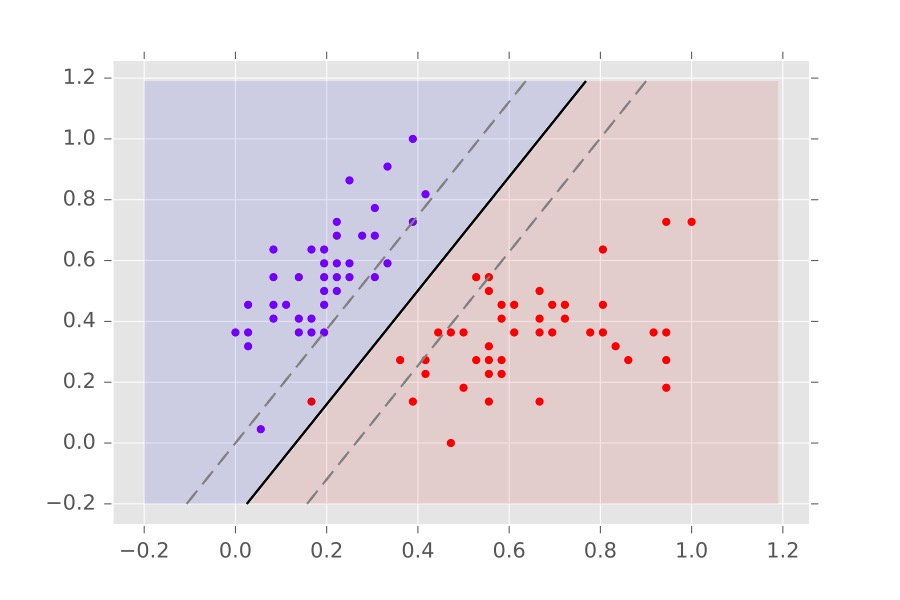
\includegraphics[width=0.5\textwidth]{slike/LinearnaMeja.jpg}}%
	\hfill % <-- Seperation
	\subcaptionbox{Polinomska meja}{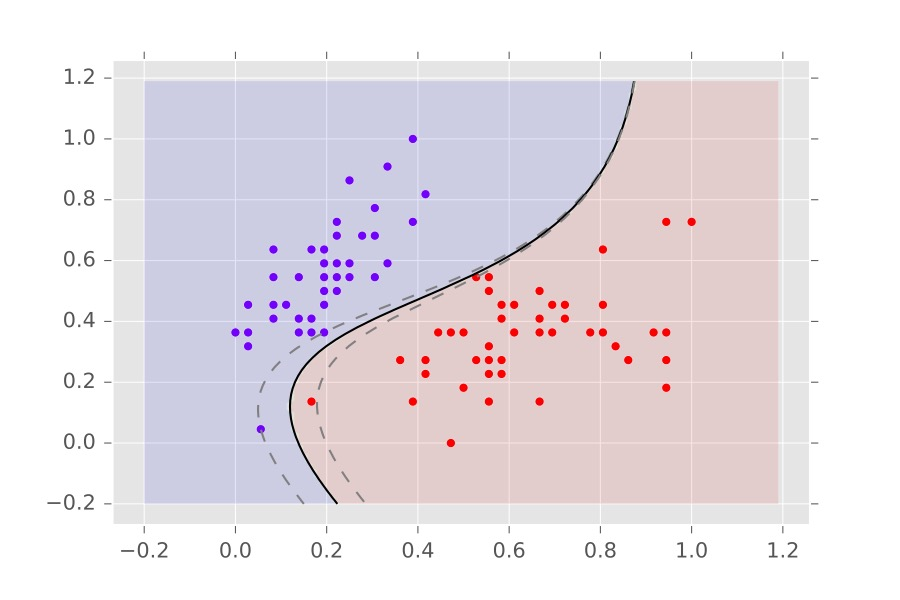
\includegraphics[width=0.5\textwidth]{slike/PolinomskaMeja.jpg}}%
	\hfill % <-- Seperation
	\\
	\subcaptionbox{Radialna meja}{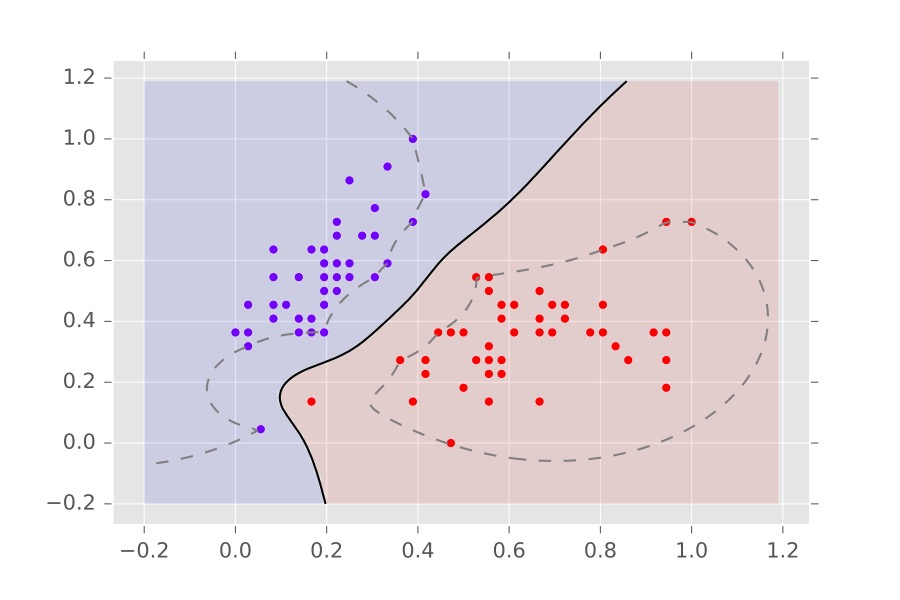
\includegraphics[width=0.5\textwidth]{slike/RadialnaMeja.jpg}}%
	\caption{Prikaz različnih modelov.}
	\label{slikaRazlicniModeli}
\end{figure}


\begin{table}[ht]
	\centering
	\begin{tabular}{llcc}
		\toprule
		& \thead{Parametri}            & \thead{Natančnost} & \thead{Število podpornih vektorjev} \\ 
		\midrule
		Linearna meja   & $C = 10$             & 0,99       & 10                          \\
		Polinomska meja & $d = 13, C = 10$     & 0,97       & 4                           \\ 
		Radialna meja   & $\gamma = 1, C = 10$ & 0,98       & 16                          \\ 
		\bottomrule
	\end{tabular}
	\caption{Prikaz različnih modelov.}
	\label{tabelaRazlicniModeli}
\end{table}

Kot vidimo, smo podatke normalizirali na interval $[0,1]$. To izvedemo z namenom, da preprečimo vpliv podajanja podatkov v različnih merskih enotah. Črna črta predstavlja ločnico med razredoma. Siva črtkana črta predstavlja predznačeno razdaljo $1$ oziroma $-1$. Rdeče točke so predstavniki enega razreda, modre pa drugega. Vsaka točka, ki leži med črtkanima črtama ali pa na nasprotni barvni podlagi, je podporni vektor. Klasifikator deluje tako, da novi meritvi pripiše rdeč razred, če točka pade na rdeče območje. Sicer ji pripiše modri razred. Natančnost modela smo v vseh treh zgornjih primerih testirali s pomočjo prečnega preverjanja z razbitjem množice na 10 enako velikih delov. Vidimo tudi, da je število podpornih vektorjev veliko manjše od števila začetnih podatkov -- teh smo imeli 100, ker smo izvzeli podatke, ki so pripadali razredu \emph{Iris-versicolor.} 

Sedaj si bomo ogledali primer s 3 razredi in uporabo metod \emph{ena na ena} in \emph{eden proti vsem}. Za podatke bomo vzeli prva dva stolpca podatkovne množice IRIS.

%%%%%%%%%%%%%%%%%%%%%%%%%%%%%%%%%%

\begin{figure}[ht]
	\centering
	\subcaptionbox{Linearna meja}{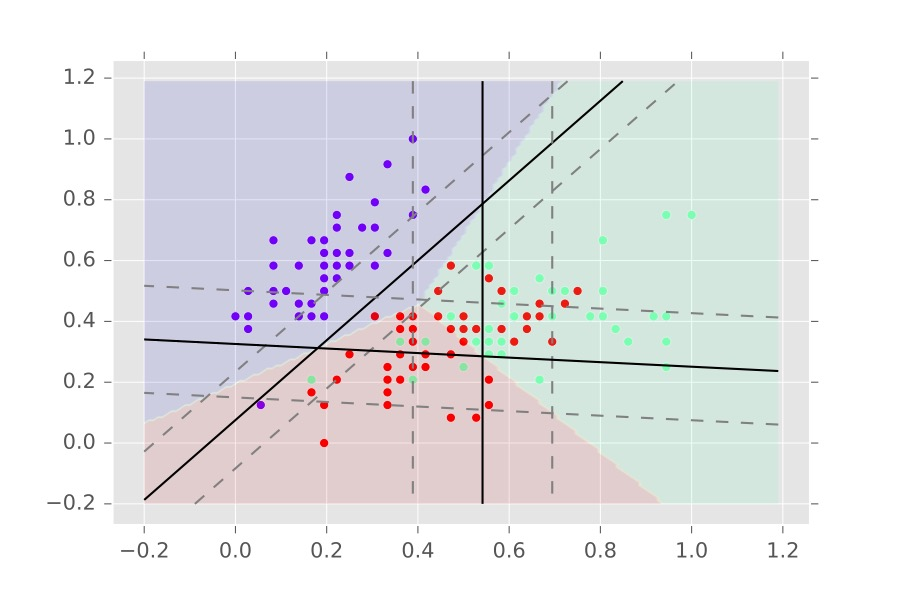
\includegraphics[width=0.5\textwidth]{slike/LinearnaMejaOVA.jpg}}%
	\hfill % <-- Seperation
	\subcaptionbox{Polinomska meja}{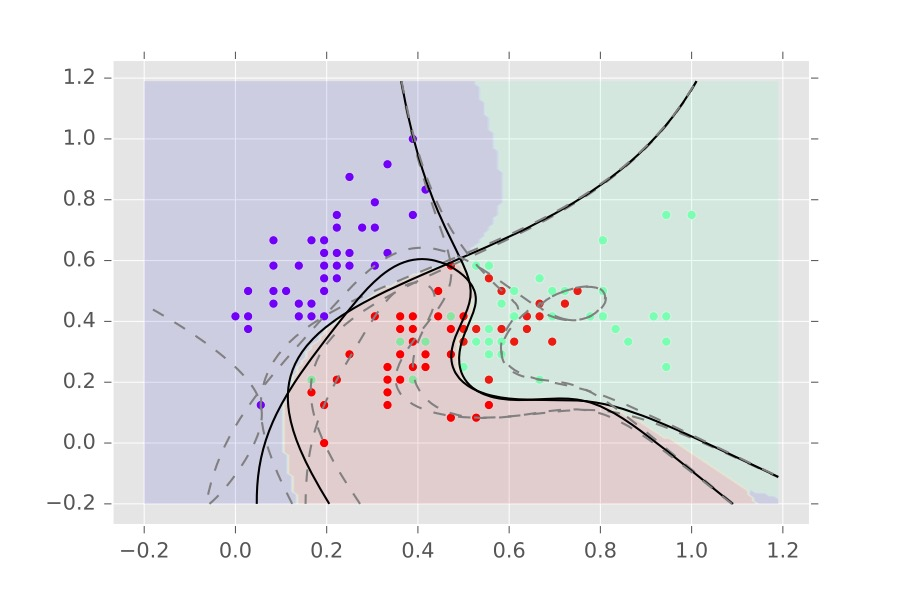
\includegraphics[width=0.5\textwidth]{slike/PolinomskaMejaOVA.jpg}}%
	\hfill % <-- Seperation
	\\
	\subcaptionbox{Radialna meja}{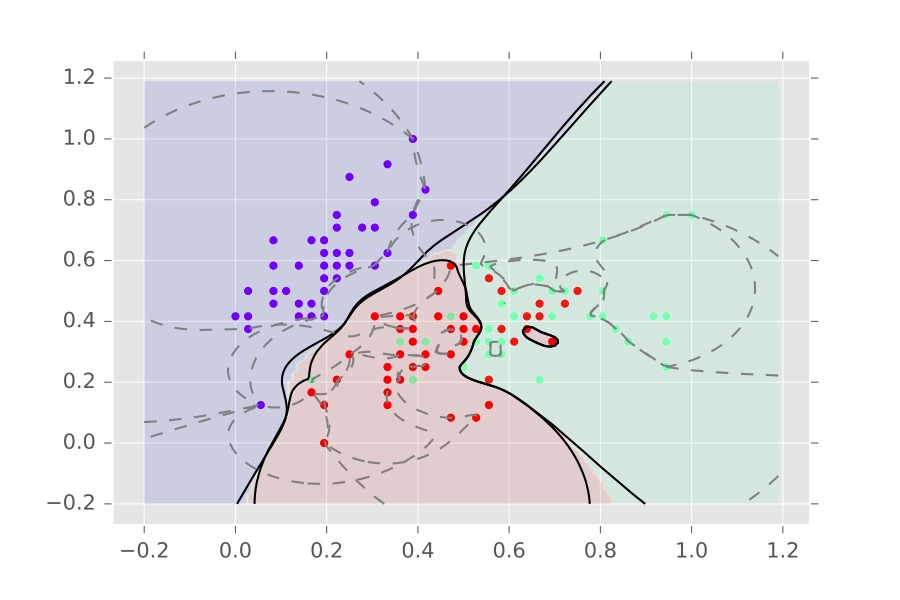
\includegraphics[width=0.5\textwidth]{slike/RadialnaMejaOVA.jpg}}%
	\caption{Prikaz različnih modelov, metoda \emph{eden proti vsem}.}
	\label{slikaRazlicniModeliOVA}
\end{figure}

\begin{table}[ht]
	\centering
	\begin{tabular}{llcc}
		\toprule
		& \thead{Parametri}            & \thead{Natančnost} & \thead{Število podpornih vektorjev} \\
		\midrule
		Linearna meja   & $C = 10$             & 0,75       & 17, 72, 93                          \\ 
		Polinomska meja & $d = 13, C = 10$     & 0,77      & 5, 66, 72                           \\ 
		Radialna meja   & $\gamma = 1, C = 10$ & 0,78       & 17, 90, 88                         \\
		\bottomrule
	\end{tabular}
	\caption{Prikaz različnih modelov, metoda \emph{eden proti vsem}.}
	\label{tabelaRazlicniModeliOVA}
\end{table}


Na sliki \ref{slikaRazlicniModeliOVA} vidimo uporabo metode \emph{eden proti vsem}, ki je opisana v poglavju \ref{poglavjeEdenProtiVsem}. Pri učenju posameznega modela smo zgradili $3$ klasifikatorje. Pri vsakem smo proglasili en razred za razred $\pr$, ostala dva pa za razred $\nr$. Tako smo dobili klasifikator, ki loči prvi razred od preostalih dveh. Nastale so tri ločitvene meje. Novi podatek klasificiramo v tisti razred, katerega klasifikator, ki loči ta razred od preostalih podatkov, vrne največjo vrednost. V sliki si to predstavljamo, da novi podatek klasificiramo v razred barvnega ozadja. S slike \ref{slikaRazlicniModeliOVA} in tabele \ref{tabelaRazlicniModeliOVA} vidimo, da je število podpornih vektorjev odvisno od prepletenosti podatkov. Bolj kot so podatki prepleteni, večje število podpornih vektorjev dobimo. V primeru polinomske meje vidimo, da smo za ločitev modrih podatkov od ostalih potrebovali 5 \emph{podpornih vektorjev}, medtem ko smo za ločitev zelenih in rdečih potrebovali bistveno več podpornih vektorjev.




%%%%%%%%%%%%%%%%%%%%%%%%%%%%%%%%%%
\begin{figure}[ht]
	\centering
	\subcaptionbox{Linearna meja}{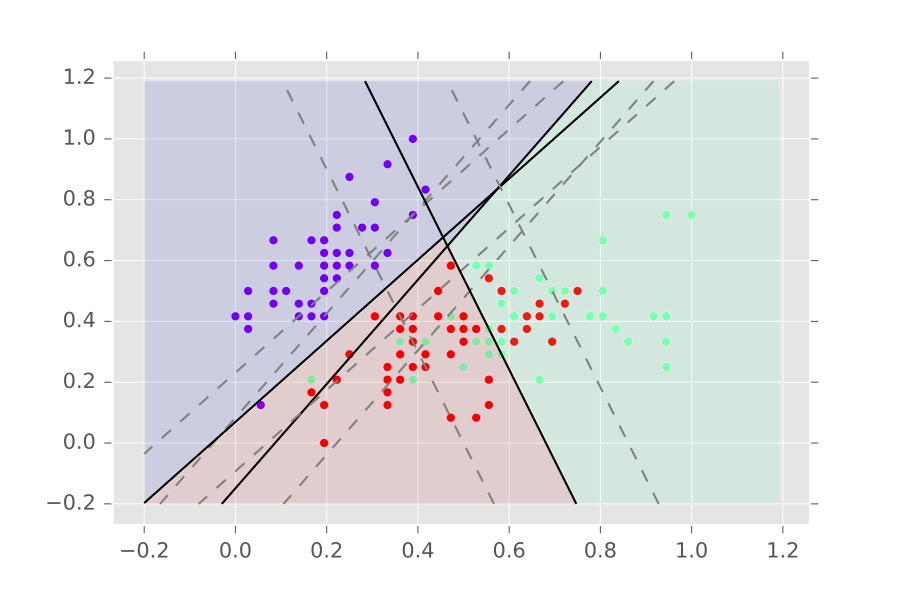
\includegraphics[width=0.5\textwidth]{slike/LinearnaMejaOVO.jpg}}%
	\hfill % <-- Seperation
	\subcaptionbox{Polinomska meja}{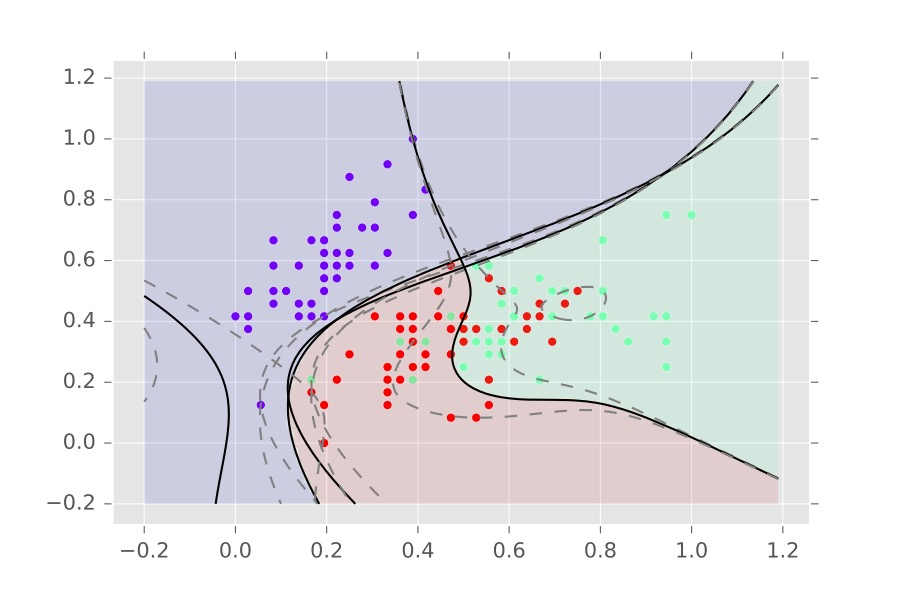
\includegraphics[width=0.5\textwidth]{slike/PolinomskaMejaOVO.jpg}}%
	\hfill % <-- Seperation
	\\
	\subcaptionbox{Radialna meja}{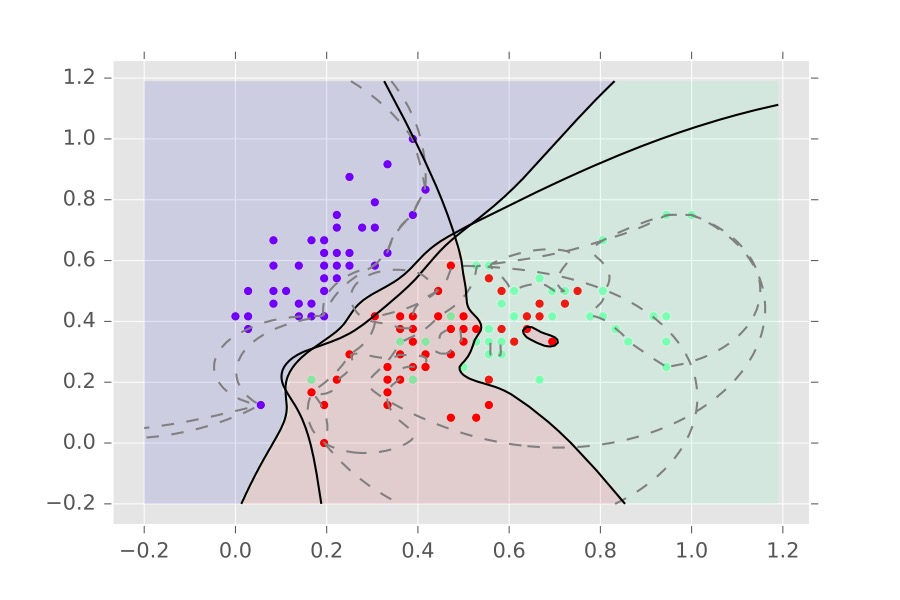
\includegraphics[width=0.5\textwidth]{slike/RadialnaMejaOVO.jpg}}%
	\caption{Prikaz različnih modelov, metoda \emph{ena na ena}.}
	\label{slikaRazlicniModeliOVO}
\end{figure}


\begin{table}[ht]
	\centering
	\begin{tabular}{cccc}
		\toprule
		& \thead{Parametri}            & \thead{Natančnost} & \thead{Število podpornih vektorjev} \\  
		\midrule
		Linearna meja   & $C = 10$             & 0,76       & 17, 12, 70                          \\ 
		Polinomska meja & $d = 13, C = 10$     & 0,79      & 4, 4, 65                        \\ 
		Radialna meja   & $\gamma = 1, C = 10$ & 0,78       & 12, 17, 85                         \\ 
		\bottomrule
	\end{tabular}
	\caption{Prikaz različnih modelov, metoda \emph{ena na ena}.}
	\label{tabelaRazlicniModeliOVO}
\end{table}


Na sliki \ref{slikaRazlicniModeliOVO} vidimo primer uporabe metode \emph{ena na ena.} V splošnem pri tej metodi dobimo $\binom{N}{2}$ število klasifikatojev za en model, kjer je $N$ število razredov. To se v primeru treh različnih razredov sklada z številom klasifikatorjev pri metodi \emph{eden proti vsem.} 
Pri obeh metodah vidimo, da se pri radialnem jedru na zelenem območju pojavi rdeč otoček. To bi lahko vzeli za primer preprileganja podatkov, saj izgleda, da področje rdečega otočka verjetno bolj pripada zelenemu razredu kot rdečemu.  

V zgornjih primerih je natančnost različnih jeder dokaj podobna. Pogosto pa dobimo podatkovno množico, na kateri kakšni tipi jeder dosežejo veliko večjo natančnost kot drugi. Oglejmo si tak primer. 


%%%%%%%%%%%%%%%%%%%%%%%%%%%%%%%%%%
\begin{figure}[ht]
	\centering
	\subcaptionbox{Linearna meja}{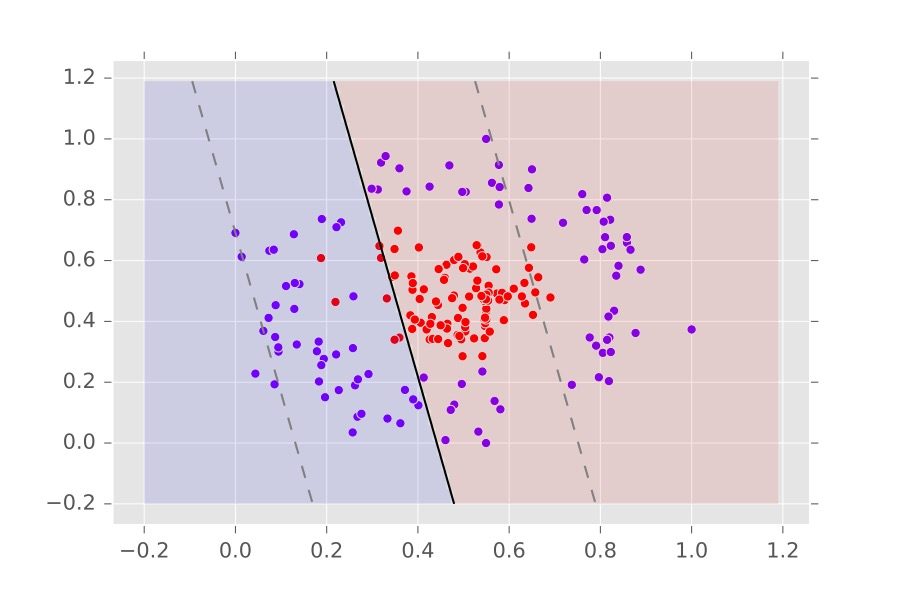
\includegraphics[width=0.5\textwidth]{slike/RadialniPodatkiLinearnaMeja.jpg}}%
	\hfill % <-- Seperation
	\subcaptionbox{Polinomska meja}{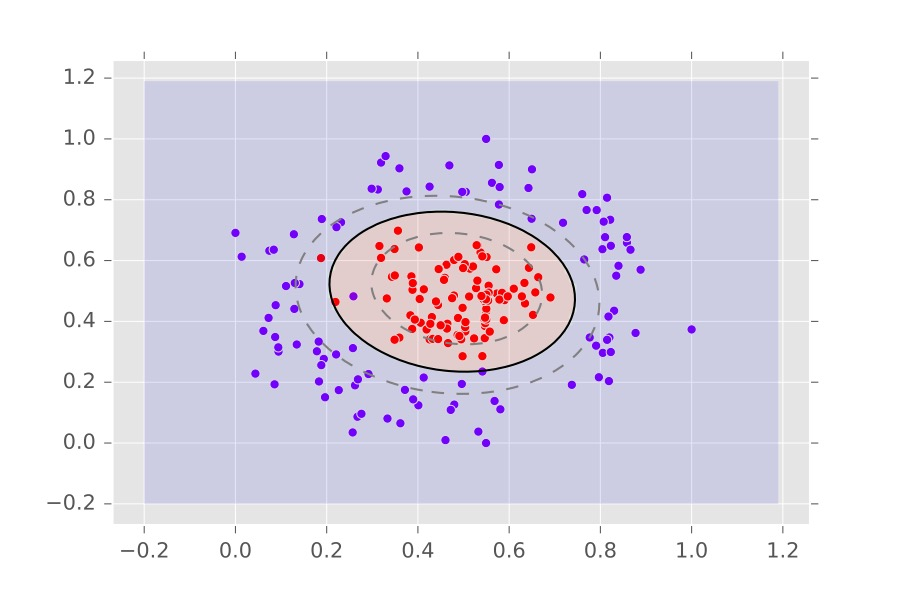
\includegraphics[width=0.5\textwidth]{slike/RadialniPodatkiPolinomskaMeja.jpg}}%
	\hfill % <-- Seperation
	\\
	\subcaptionbox{Radialna meja}{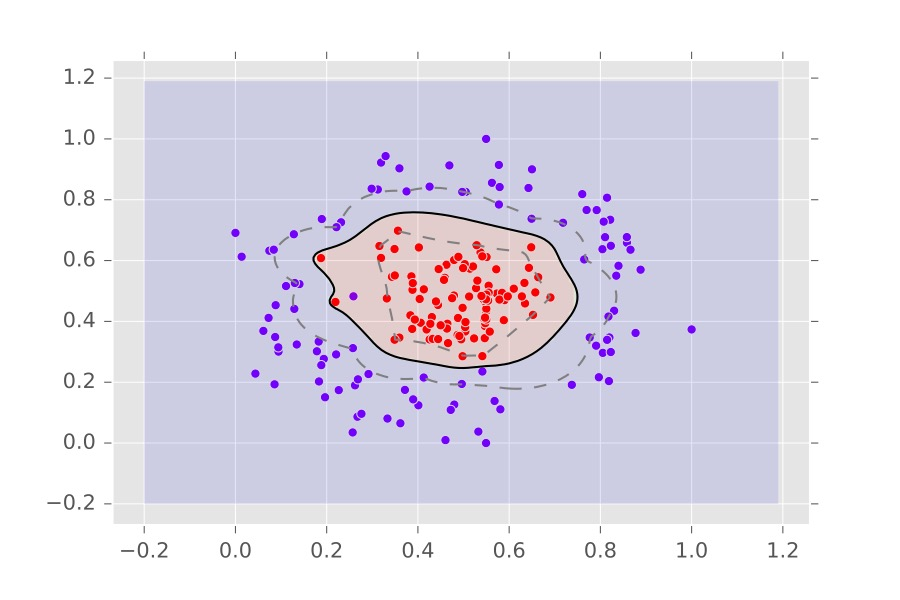
\includegraphics[width=0.5\textwidth]{slike/RadialniPodatkiRadialnaMeja.jpg}}%
	\caption{Prikaz različnih modelov, kjer je velika razlika v natančnosti.}
	\label{slikaRazlikaVNatancnosti}
\end{figure}


\begin{table}[ht]
	\centering
	\begin{tabular}{llcc}
		\toprule
		& \thead{Parametri}            & \thead{Natančnost} & \thead{Število podpornih vektorjev} \\ 
		\midrule 
		Linearna meja   & $C = 10$             & 0,59       &  193                        \\ 
		Polinomska meja & $d = 4, C = 10$     & 0,98      & 28                       \\ 
		Radialna meja   & $\gamma = 1, C = 10$ & 0,98       & 30                        \\ 
		\bottomrule
	\end{tabular}
	\caption{Prikaz različnih modelov, kjer je velika razlika v natančnosti.}
	\label{tabelaRazlikaVNatancnosti}
\end{table}

Na sliki \ref{slikaRazlikaVNatancnosti} vidimo, da vsa jedra niso primerna za vse podatke. Na umetno zgeneriranih 200 podatkih doseže linearno jedro zelo slabo natančnost. Tudi število podpornih vektorjev je zelo veliko, kar nakazuje, da je imelo linearno jedro velike težave pri določitvi meje med podatki. Po drugi strani polinomski in radialni problem nimata težav pri določitvi ločitvene meje. 

Sedaj si bomo ogledali primer, ki bo razložil, kaj točno pomeni \emph{preprileganje.} Modele bomo učili na prvih dveh stolpcih podatkovne množice IRIS, ki ji bomo odvzeli podatke, ki pripadajo razredu \emph{Iris-setosa}. 

%%%%%%%%%%%%%%%%%%%%%%%%%%%%%%%%%%
\begin{figure}[ht]
	\centering	
	\subcaptionbox{Radialna meja 1}{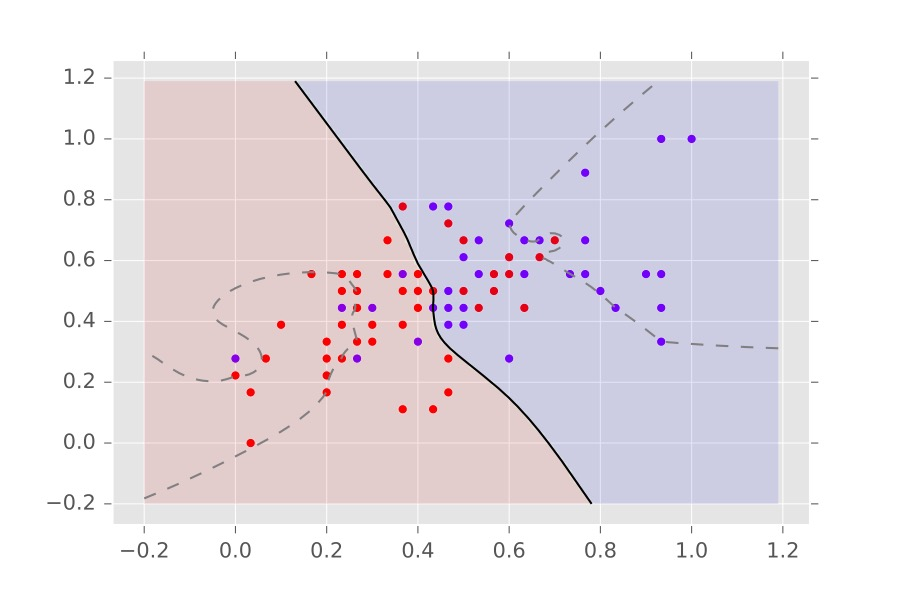
\includegraphics[width=0.5\textwidth]{slike/RadialnaMejaGamma01.jpg}}%
	\hfill % <-- Seperation
	\subcaptionbox{Radialna meja 2}{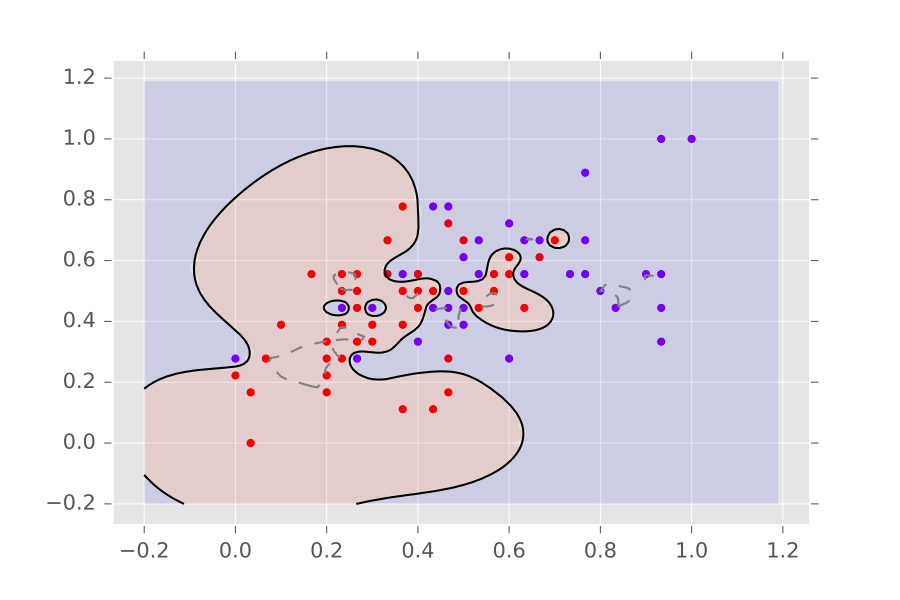
\includegraphics[width=0.5\textwidth]{slike/RadialnaMejaGamma10.jpg}}%
	\hfill % <-- Seperation
	\\
	\subcaptionbox{Radialna meja 3}{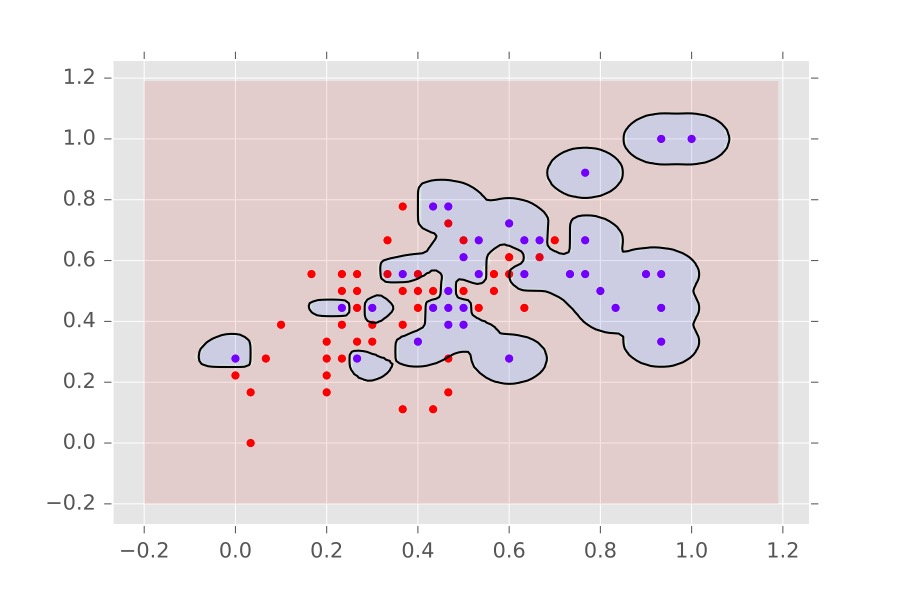
\includegraphics[width=0.5\textwidth]{slike/RadialnaMejaGamma100.jpg}}%
	\caption{Prikaz različnih modelov, ki ilustrirajo \emph{preprileganje}.}
	\label{slikaPreprileganje}
\end{figure}


\begin{table}[ht]
	\centering
	\begin{tabular}{llccc}
		\toprule
		& \thead{Parametri}            & \thead{Natančnost} & \thead{Natančnost na\\ učni množici} & \thead{Število \\ podpornih vektorjev} \\ 
		\midrule 
		Radialna meja 1 &$\gamma = 0{,}1 ; C = 10$        & 0,72  & 0,75     &  80                        \\ 
		Radialna meja 2 &  $\gamma = 10; C = 10$    & 0,58   & 0,89   & 95                       \\ 
		Radialna meja  3 & $\gamma = 100; C = 10$ & 0,48    & 0,89   & 100                        \\ 
		\bottomrule
	\end{tabular}
	\caption{Prikaz različnih modelov, ki ilustrirajo \emph{preprileganje}.}
	\label{tabelaPreprileganje}
\end{table}

Na sliki \ref{slikaPreprileganje} vidimo obnašanje radialnega jedra pri treh različnih parametrih $\gamma$ na danih podatkih. Z večanjem parametra $\gamma$ natančnost na učni množici raste, vendar se model preveč prilega samim podatkom, zato njegova natančnost, izračunana z metodo \emph{prečnega preverjanja}, pada. Pri $\gamma = 100$ se model že tako preveč prilega podatkom, da je njegova natančnost približno 0,5. Tako natančnost lahko dosežemo tudi z naključnim modelom, zato ta model ni dober. V zgornjem primeru bi za končni model izbrali prvi model, saj vrne največjo natančnost. Na poljubnih podatkih ne vemo v naprej, s kakšnimi parametri bomo dosegli največjo natančnost, zato moramo testirati več modelov, na koncu pa izberemo tistega, za katerega smo ocenili, da bodo njegove napovedi najbolj točne. 


\subsection{Večja podatkovna množica}
Sedaj bomo naučili model na malo večji podatkovni množici. Naslov podatkov je \emph{Izbira kontracepcijskih metod}. Podatki so zbrani iz nacionalne ankete o razširjenosti kontracepcije v Indoneziji iz leta 1987. Vzorci so poročene ženske, ki v času razgovora niso bile noseče, oziroma niso vedele, da so. Cilj je napovedati kontracepcijsko metodo za žensko (brez uporabe, dolgoročna uporaba ali kratkoročna uporaba) na podlagi njenih demografskih in socialno-ekonomskih značilnostih. Slednje značilnosti so:
\begin{enumerate}
	\item
	Starost ženske (številski podatek)
	\item
	Njena izobrazba (1--4, kjer je 1 nizka in 4 visoka)
	\item 
	Moževa izobrazba (1--4, kjer je 1 nizka in 4 visoka)
	\item 
	Število rojenih otrok (številski podatek)
	\item 
	Možev poklic (štirje različni kategorični podatki, ki jih označimo z 1--4)
	\item 
	Življenjski standard (1--4, kjer je 1 nizek in 4 visok)
\end{enumerate}
Napovedujemo, kakšno kontracepcijsko metodo ženska uporablja. Izbiramo med tem, da je ne uporablja, da jo uporablja dolgoročno, da jo uporablja kratkoročno. Število vzorcev je $1473$. Oglejmo si graf, ki predstavlja različne modele, ki temeljijo na polinomskem jedru. 
\begin{figure}[ht]
	\centering
	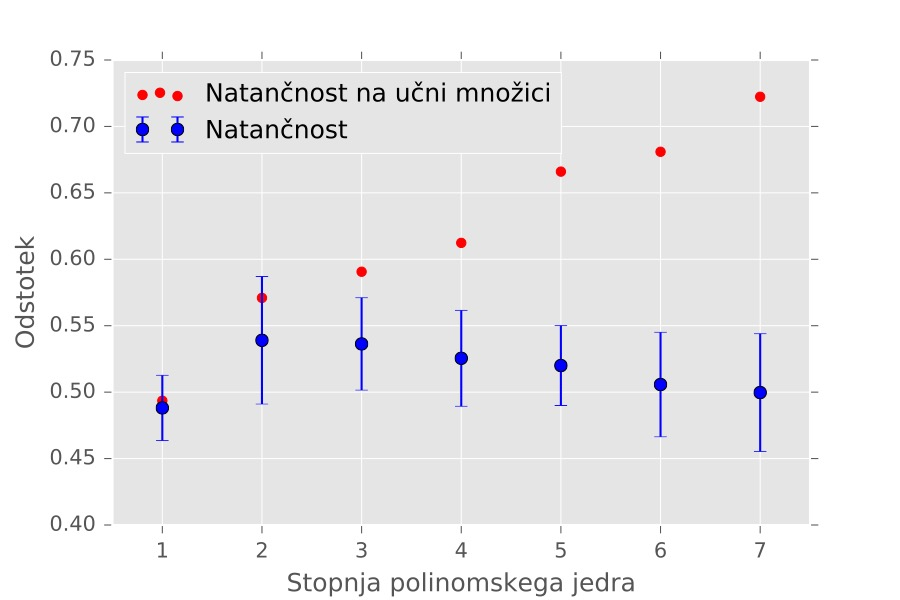
\includegraphics[width=0.70\textwidth]{slike/Natancnost.jpg}
	\caption{Prikaz različnih modelov, naučenih na izbranih podatkih.}
	\label{slikaNatancnostPolinom}
\end{figure}
Na podatkih smo uporabili različna polinomska jedra. Parameter cene smo nastavili na $C = 10$, uporabili smo metodo \emph{ena na ena} za večrazredne podatke. Z modro je označena natančnost, ki smo jo pridobili z uporabo \emph{prečnega preverjanja}, kjer smo začetno množico razdelili na $8$ podskupin. Z rdečo je označena natančnost, ki jo model doseže na celih podatkih. Vidimo, da natančnost na učni množici raste z višanjem stopnje polinomske ločitvene krivulje. Hkrati opazimo, da s polinomskim jedrom stopnje 2 dosežemo največjo natančnost s prečnim preverjanjem. V tem primeru bi za končni model izbrali polinomsko jedro stopnje 2. Polinomski modeli višje stopnje se preveč prilegajo samim podatkom, zato natančnost, dobljena s prečnim preverjanjem, pada. Po drugi strani pa je linearen model precej slabši od kvadratnega. Zato izberemo polinomski model stopnje 2. Vidimo, da je v tem primeru natančnost modela približno 0,55. Izračunajmo, kakšna bi bila natančnost naključne napovedi, pri napovedovanju 3 različnih možnih razredov, za katere vemo, da imajo zaporedoma 629, 333 in 511 predstavnikov. Za najboljšo možno naključno napoved maksimiziramo
\begin{align*}
	&\frac{629}{1473}p + \frac{333}{1473}q + \frac{521}{1473}r, \\
	\text{pri pogojih:}~&p + q + r = 1, p \ge 0, q \ge 0, r \ge 0. 
\end{align*} 
Trojica, ki reši to optimizacijsko nalogo, je $(p,q,r) = (1, 0, 0)$. V tem primeru dobimo natančnost 0,42702. Takemu klasifikatorju, ki vedno napove večinski razred, pravimo \emph{večinski klasifikator}. Vidimo, da naš model napove ciljno spremenljivko z večjo natančnostjo.

\begin{table}[H]
	\centering
	\begin{tabular}{cc}
		\toprule
		\thead{Stopnja \\ polinomskega jedra}  & \thead{Čas učenja [s] } \\ 
		\midrule 
		1                          & 20,38                     \\ 
		2                          & 19,56                     \\ 
		3                          & 18,55                      \\ 
		4                          & 21,26                     \\ 
		5                          & 27,37                     \\ 
		6                          & 30,94                   \\ 
		7                          & 43,28                    \\ 
		\bottomrule
	\end{tabular}
	\caption{Trajanje učenja modelov.}
	\label{tabelaUcenjeModelov}
\end{table}

Zanimivo je videti tudi čas učenja posameznih polinomskih modelov. Vidimo, da so časi vseh izbranih modelov približno enakih velikostnih razredov. To smo dosegli s prevedbo problema na dualni problem, kjer nas namesto preslikanega prostora zanima samo skalarni produkt v preslikanem prostoru. Razlog, da višja jedra porabijo nekoliko več časa, bi lahko bila počasnejša konvergenca optimizacijskega algoritma k rešitvi. 


\section*{Dodatek A: Programska koda}
V dodatku se nahaja programska koda, ki je bila napisana za namene diplomske naloge ter s pomočjo katere so nastali zgornji primeri uporabe. Koda je prosto dostopna tudi na spletnem naslovu \url{github.com/lenarttreven/Diploma/tree/master/diplomaKoda}.


\begin{scriptsize}

\begin{minted}[
 breaklines,
 mathescape,
 numbersep=5pt,
 frame=single,
 ]{python}

import matplotlib.pyplot as plt
from matplotlib import style
import numpy as np
import pandas as pd
from cvxpy import *
from sklearn.utils import shuffle

style.use('ggplot')

class SVM():
def __init__(self, data, kernel="linear", degree=1, g=100, k1=1, k2=1, C=50, method='ovo'):
    self.K = self.make_k(kernel, degree, g, k1, k2)
    self.kernel = kernel
    self.degree = degree
    self.g = g
    self.k1 = k1
    self.k2 = k2
    self.C = C
    self.method = method
    self.myfit, self.mypredict = self.make_environment()
    self.prepare_data(data)
    self.data = data.copy()
    self.normalized_data = normalize_df(data)
    self.maximum = np.array(self.data[self.data.columns.difference(['razred'])].max())
    self.minimum = np.array(self.data[self.data.columns.difference(['razred'])].min())
 
def make_k(self, kernel, degree=1, g=100, k1=1, k2=1): 
    if kernel == 'linear':
        def jedro(x1, x2):
            return np.dot(x1, x2)
        return jedro
    elif kernel == 'polynomial':
        def jedro(x1, x2):
            return (1 + np.dot(x1, x2)) ** degree
        return jedro
    elif kernel == 'radial':
        def jedro(x1, x2):
            return np.exp(-g * np.linalg.norm(x1 - x2, axis=-1))
        return jedro
    elif kernel == 'neural':
        def jedro(x1, x2):
            return np.tanh(k1 * np.dot(x1, x2)+ k2) 
        return jedro

def make_environment(self): 
    if self.method == 'ovo':
        def fit_one_versus_one(dataset=None):
            if dataset is None:
                dataset = self.normalized_data
            napovedi = dict()
            for i in range(self.stevilo_razredov):
                for j in range(i):
                    data = dataset.loc[dataset['razred'].isin([i, j])]
                    X = np.array(data.drop(['razred'], 1)).astype(np.float)
                    y = np.array(data['razred']).astype(np.float)
                    y[y == j] = -1
                    y[y == i] = 1
                    a, b, indeksi = self._fit(X, y)
                    napovedi[(i,j)] = (a, b, indeksi)
            return napovedi
        
        def predict_one_versus_one(X, napovedi, dataset=None):
            if dataset is None:
                dataset = self.normalized_data
            glasovi = np.zeros(self.stevilo_razredov)
            for i in range(self.stevilo_razredov):
                for j in range(i):
                    data = dataset.loc[dataset['razred'].isin([i, j])]
                    X_data = np.array(data.drop(['razred'], 1)).astype(np.float)
                    y_data = np.array(data['razred']).astype(np.float)
                    y_data[y_data == j] = -1
                    y_data[y_data == i] = 1
                    glas = self._predict(X, X_data, y_data, *napovedi[(i,j)])
                    if glas == 1:
                        glasovi[i] += 1
                    else:
                        glasovi[j] += 1
            return np.argmax(glasovi)
        return fit_one_versus_one, predict_one_versus_one
    
    elif self.method == 'ova':
        def fit_one_versus_all(dataset=None):
            if dataset is None:
                dataset = self.normalized_data
            napovedi = dict()
            for i in range(self.stevilo_razredov):
                X_train = np.array(dataset.drop(['razred'], 1)).astype(np.float)
                y_train = np.array(dataset['razred']).astype(np.float)
                y_train[y_train != i] = -1
                y_train[y_train == i] = 1
                napovedi[i] = self._fit(X_train, y_train)
            return napovedi
        def predict_one_versus_all(X, napovedi, dataset=None):
            if dataset is None:
                dataset = self.normalized_data
            glasovi = np.zeros(self.stevilo_razredov)
            for i in range(self.stevilo_razredov):
                X_data = np.array(dataset.drop(['razred'], 1)).astype(np.float)
                y_data = np.array(dataset['razred']).astype(np.float)
                y_data[y_data != i] = -1
                y_data[y_data == i] = 1
                glasovi[i] = self.classifier(X, X_data, y_data, *napovedi[i])
            return np.argmax(glasovi)
        return fit_one_versus_all, predict_one_versus_all
    else: 
        raise ValueError('No such method is known to this program. Try ovo (one versus one) or ova (one versus all)')
        
def prepare_data(self, df):
    self.stevilo_razredov = df.razred.nunique()
    self.to_indeks = dict()
    self.to_name = dict()
    for indeks, name in enumerate(df.razred.unique()):
        self.to_indeks[name] = indeks
        self.to_name[indeks] = name
    df.replace(self.to_indeks, inplace=True)
                  
def fit(self):
    self.napovedi = self.myfit()
    X = np.array(self.normalized_data.drop(['razred'], 1)).astype(np.float)
    y = np.array(self.normalized_data['razred']).astype(np.float)
    self.accuracy_on_set = self.test(X, y, self.napovedi, self.normalized_data)

def cross_validate(self, k=10):
    self.split_data = split_data(self.data, k)
    results = []
    tests = []
    for i in range(k):
        test = self.split_data[i]
        train = pd.concat([df for num, df in enumerate(self.split_data) if not num == i])
        maximum = np.array(train[train.columns.difference(['razred'])].max())
        minimum = np.array(train[train.columns.difference(['razred'])].min())
        train = normalize_df(train)
        test_X = np.array(test.drop(['razred'], 1)).astype(np.float)
        test_y = np.array(test['razred']).astype(np.float)
        test_X = (test_X - minimum) / (maximum - minimum)
        napovedi = self.myfit(dataset=train)
        accuracy = self.test(test_X, test_y, napovedi, train)
        results.append((napovedi, accuracy))
        tests.append(accuracy)
    self.results = results
    self.accuracy_test = np.array(tests)
    self.accuracy = np.mean(self.accuracy_test)
    self.izracunaj_standarni_odklon_natancnosti()
       
def test(self, X, y, napovedi, dataset):
    all_instances = 0
    correct_instances = 0
    for index, instance in enumerate(X):
        all_instances += 1
        if self.mypredict(instance, napovedi, dataset=dataset) == y[index]:
            correct_instances += 1
    accuracy = correct_instances/all_instances
    return accuracy

def izracunaj_standarni_odklon_natancnosti(self):
    vzorci = self.accuracy_test
    povprecje = self.accuracy
    n = len(vzorci)
    varianca = 0
    for i in vzorci:
        varianca += (i - povprecje)**2
    varianca /= n
    self.standarni_odklon_natancnosti = np.sqrt(varianca)
      
def predict(self, X, df, ydf, a, b):
    X = (X - self.minimum) / (self.maximum - self.minimum)
    return self._predict(X, df, ydf, a, b)

def _predict(self, X, df, ydf, a, b, indeksi):
    return np.sign(self.classifier(X, df, ydf, a, b, indeksi))

def posplosen_skalarni_produkt(self, x_j, X, y, alpha, indeksi):
    rezultat = 0
    for i in indeksi: 
        rezultat += alpha[i] * y[i] * self.K(x_j, X[i])
    return rezultat
    
def find_support_vectors(self, alpha,X, y, odpad= 10 ** (-5), odstopanje=0.99):
    a = np.amax(alpha)
    #poiščemo indkse, za katere so X[i] podporni vektorji
    indeksi = []
    for i in range(len(alpha)):
        if alpha[i]/a >= odpad:
            indeksi.append(i)
    #sedaj določimo b, ki ga potrebujemo za napoved.
    #B je vektor, ki ga bomo polnili z različnimi b-ji nato pa izračunalil njigevo povprečje
    B = []
    for i in indeksi:
        if alpha[i] < self.C * odstopanje:
            B.append(y[i] - self.posplosen_skalarni_produkt(X[i], X, y, alpha, indeksi))
    
    b = np.mean(B)
    return (b, indeksi)
     
def classifier(self, X, Xdf, ydf, a, b, indeksi):
    result = self.posplosen_skalarni_produkt(X, Xdf, ydf, a, indeksi)
    return result + b

def visualize(self, h=0.5):
    if len(self.data.columns) != 3:
        return 'Number of attribute dimensions is not 2'
    self.fig = plt.figure()
    self.ax = self.fig.add_subplot(1,1,1)
    df = self.normalized_data
    
    #narišemo vse različne razrede kot scatter graf:
    seznam_razredov = df.razred.unique()
    x_stolpec, y_stolpec = df.columns.difference(['razred'])

    n = len(seznam_razredov)       
    color=iter(plt.cm.rainbow(np.linspace(0,1,n)))
    
    
    for razred in seznam_razredov:
        data = df.loc[df['razred'] == razred]
        c=next(color)
        self.ax.scatter(data[x_stolpec], data[y_stolpec], c=c)
    
    #risanje crt
    h = .01  # velikost koraka v mrezi
    x_min, x_max = -0.2, 1.2
    y_min, y_max = -0.2, 1.2
    xx, yy = np.meshgrid(np.arange(x_min, x_max, h), np.arange(y_min, y_max, h))
    
    #narišemo vse meje med posameznimi razredi:
    if self.method == 'ovo':
        for i in range(self.stevilo_razredov):
            for j in range(i):
                data = self.normalized_data.loc[self.normalized_data['razred'].isin([i, j])]
                data = self.normalized_data.loc[self.normalized_data['razred'].isin([i, j])]
                Xdf = np.array(data.drop(['razred'], 1)).astype(np.float)
                ydf = np.array(data['razred']).astype(np.float)
                ydf[ydf != i] = -1
                ydf[ydf == i] = 1

                # Narisemo mejo. 
                Z = self.classifier(np.c_[xx.ravel(), yy.ravel()], Xdf, ydf, *self.napovedi[(i,j)])
                Z = Z.reshape(xx.shape)
                plt.contour(xx, yy, Z, levels=[-1 , 0, 1], colors=('grey', 'black', 'grey'), linestyles=('dashed', 'solid', 'dashed'))
    
    if self.method == 'ova':
        for i in range(self.stevilo_razredov):
            Xdf = np.array(df.drop(['razred'], 1)).astype(np.float)
            ydf = np.array(df['razred']).astype(np.float)
            ydf[ydf != i] = -1
            ydf[ydf == i] = 1
            
            # Narisemo mejo.
            Z = self.classifier(np.c_[xx.ravel(), yy.ravel()], Xdf, ydf, *self.napovedi[i])
            Z = Z.reshape(xx.shape)
            plt.contour(xx, yy, Z, levels=[-1 , 0, 1], colors=('grey', 'black', 'grey'), linestyles=('dashed', 'solid', 'dashed'))
    
    X = np.c_[xx.ravel(), yy.ravel()]
    Z = np.zeros(len(X))
    for index, i in enumerate(X):
        Z[index] = self.mypredict(i, self.napovedi)
    Z = Z.reshape(xx.shape)
    plt.contourf(xx, yy, Z, alpha=0.1)
    plt.show()
    
def _fit(self, X, y):
    n = len(X)
    m = len(X[0])

    a = Variable(n)

    # Postavimo optimizacijski model
    A = np.zeros(shape=(n,n))
    for i in range(n):
        for j in range(n):
            A[i][j] = self.K(X[i], X[j])
    obj = Maximize(sum_entries(a) - 1/2 * quad_form(a, np.dot(np.dot(np.diag(y), A), np.diag(y))))
    constraints = [a >= 0,  a <= self.C, a.T * y == 0]
    
    prob = Problem(obj, constraints)
    prob.solve()

    a = np.squeeze(np.asarray(a.value))
    b, indeksi = self.find_support_vectors(a, X, y, odpad=10**(-5), odstopanje=0.99)
    return (a, b, indeksi)
    
def normalize_df(df):
    df[df.columns.difference(['razred'])] = df[df.columns.difference(['razred'])].apply(lambda x: (x - x.min()) / (x.max() - x.min())) 
    return df    
    
def normalize_arr(X):
    X_normed = (X - X.min(0)) / X.ptp(0)
    return X_normed
    
def split_data(data, k=10):
    data = shuffle(data)
    data.reset_index(drop=True,inplace=True)
    split_data = partition(data, k)
    return split_data
        
def partition(lst, n):
    division = len(lst) / n
    return [lst[round(division * i):round(division * (i + 1))] for i in range(n)]

\end{minted}
\end{scriptsize}






\section*{Slovar strokovnih izrazov}

\geslo{bootstrapping}{zankanje}
\geslo{cross-validation}{prečno preverjanje}
\geslo{kernel}{jedro}
\geslo{overfitting}{preprileganje}
\geslo{support vector}{podporni vektor}

% seznam uporabljene literature
\begin{thebibliography}{99}


\bibitem{ITNO}
A.~Beck, \emph{Introduction to nonlinear optimization: theory, algorithms, and applications with MATLAB}, MOS-SIAM Series on Optimization \textbf{19}, Society for Industrial and Applied Mathematics, 	Philadelphia, 2014.
\bibitem{DM}
E.~Frank in I.~H.~Witten, \emph{Data mining: practical machine learning tools and techniques}, Morgan Kaufmann series in data management systems, Morgan Kaufmann, Amsterdam, 2005.
\bibitem{ESL}
J.~Friedman, T.~Hastie in  R.~Tibshirani, \emph{The elements of statistical learning: data mining, inference, and prediction}, Springer series in statistics, Springer, New York, 2. izd., 2009.
\bibitem{AITSL}
T.~Hastie, G.~James, R.~Tibshirani in D.~Witten, \emph{An introduction to statistical learning: with applications in R}, Springer texts in statistics \textbf{103}, Springer, New York, 2013. 
\bibitem{RKHS}
D.~Hush, C.~Scovel in I.~Steinwart, \emph{An explicit description of the reproducing kernel hilbert spaces of gaussian RBF kernels}, IEEE Trans.\ Inform.\ Theory \textbf{52} (2006) 4635--4643.
\bibitem{Mercer}
J.~Thickstun, \emph{Mercer's theorem}, [ogled 13.~6.~2018], dostopno na \url{homes.cs.washington.edu/~thickstn/docs/mercer.pdf}.



\end{thebibliography}

\end{document}

